\chapter{Method}\label{chapter:method}
This section covers the principles and design decisions behind each feature.

% ----------------------------- %
% ------ SCAN SIMULATION ------ %
% ----------------------------- %

\section{Scan Simulation}\label{method:scan_simulation}
The scan simulation works by resampling the perfect scan supplied. Each point in the simulation is a result of linearly interpolating a point in the original.

The point that is sampled is determined by the dimensions, resolution, center and direction of the scan. Firstly the $origin$ (location of pixel (0, 0, 0)) is computed from the $center$.

\begin{align*}
origin = center \text{ }-\text{ }& xDir * \frac{(scanWidth * xResolution)}{2} \nonumber \\
 	  			\text{ }-\text{ }& yDir * \frac{(scanHeight * yResolution)}{2} \nonumber \\
 	  			\text{ }-\text{ }& zDir * \frac{(numSlices * zResolution)}{2} \nonumber \\
 	  			\\
	\text{where}& \\
	& scanWidth \text{ - number of pixels/slices in simulated scan slice} \nonumber \\
	& scanHeight \nonumber \\
	& numSlices \nonumber \\
	& xResolution \text{ - the size of each simulated pixel} \nonumber \\
	& yResolution \text{\hspace*{1.5em} (in pixels - relative to reconstruction)} \nonumber \\
	& zResolution \nonumber \\
	& xDir \text{ - the direction vectors of the simulated scan} \nonumber \\
	& yDir \nonumber \\
	& zDir \nonumber
\end{align*}

Then point $p$ in the simulated scan can be mapped to sample point $s$:

\begin{align*}
	 s = origin \text{ }+\text{ }& xDir * (p[x] * xResolution) \nonumber \\
 	  			\text{ }+\text{ }& yDir * (p[y] * yResolution) \nonumber \\
 	  			\text{ }+\text{ }& zDir * (p[z] * zResolution) \nonumber \\ 	  			
\end{align*}

Note that the point $s$ is a continuous index. e.g. a 5 pixel image can be interpolated in the range [-0.5, 4.5].

The simulation is acquired slice by slice and each slice can optionally be corrupted with motion. A transformation matrix, $T$, is generated for each slice which represents a rotation of a random number of degrees (up to a max) about a random axis. When enabled the point $T(s)$ is sampled instead of $s$. If the transform moves $s$ out of the volume then the value is 0. Figure \ref{fig:scan_simulation_movement_comparison} shows the effect of changing the maximum rotation angle.

\begin{figure}[H]
  \centering
  \begin{subfigure}[b]{0.32\textwidth}
    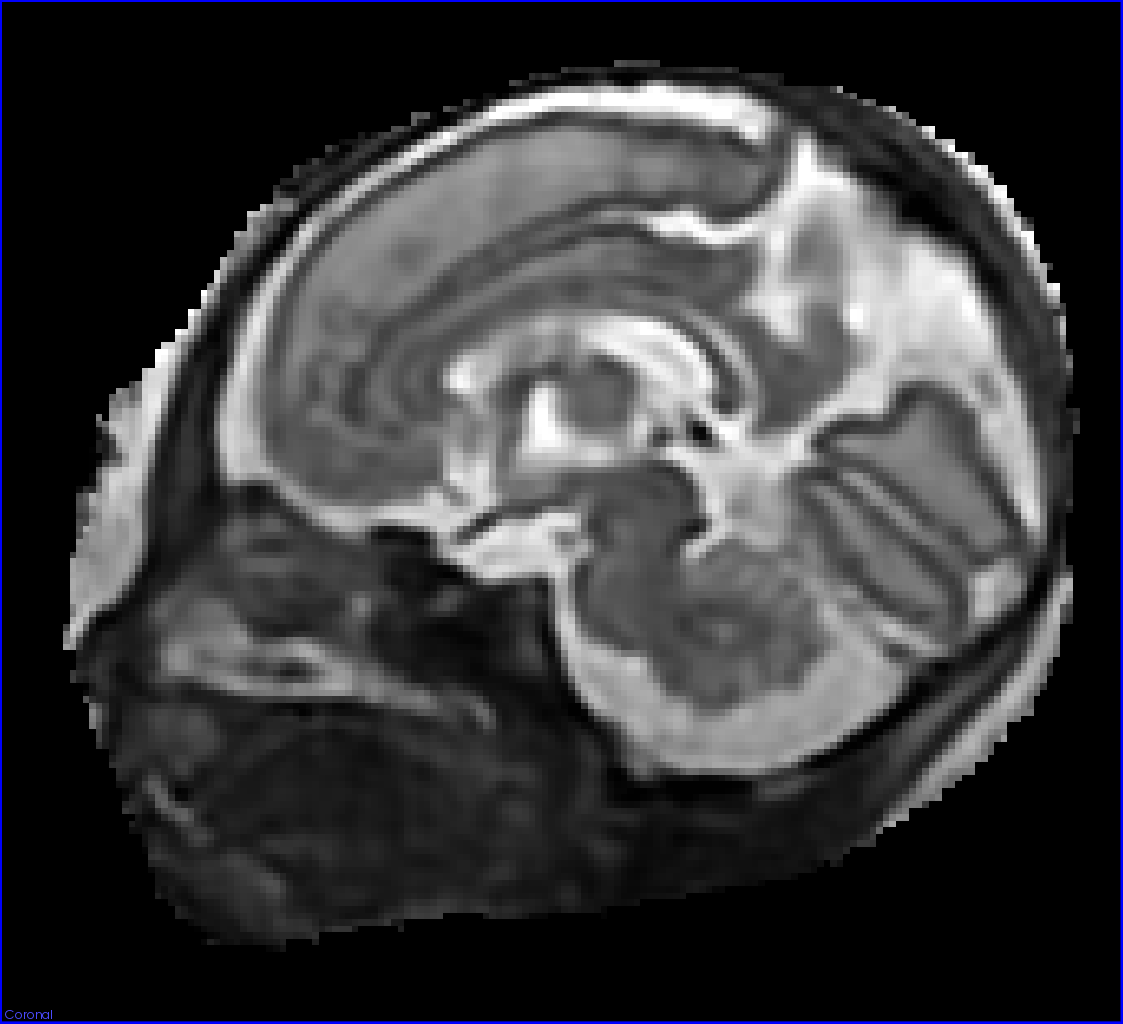
\includegraphics[width=\textwidth]{images/scan_simulation/scan_simulation_no_movement.png}
    \caption{No Movement}\label{fig:scan_simulation_no_movement}
  \end{subfigure}%
  ~ %add desired spacing between images, e. g. ~, \quad, \qquad, \hfill etc.
    %(or a blank line to force the subfigure onto a new line)
  \begin{subfigure}[b]{0.32\textwidth}
    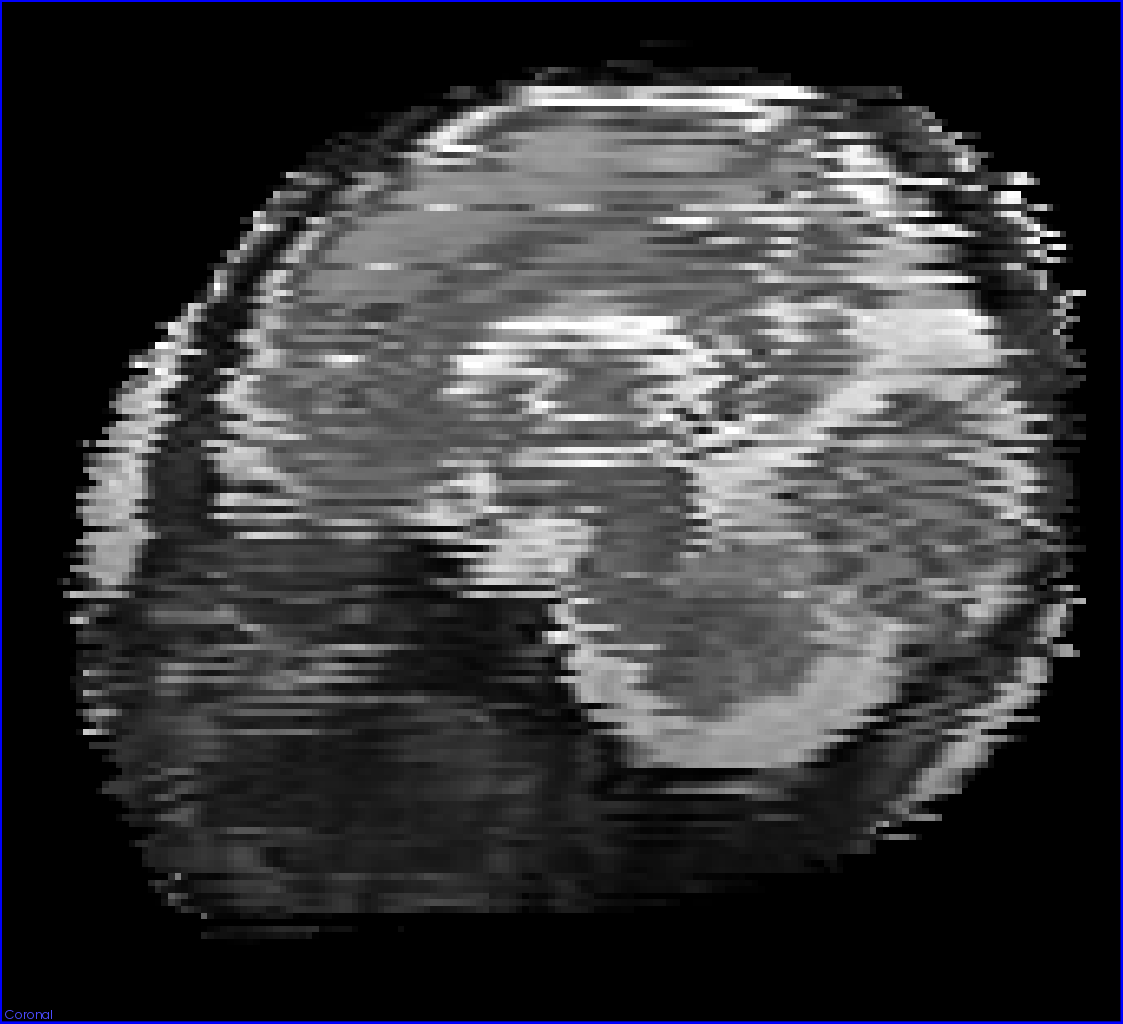
\includegraphics[width=\textwidth]{images/scan_simulation/scan_simulation_5.png}
    \caption{5 Degrees}\label{fig:scan_simulation_5_degrees}
  \end{subfigure}%
  ~ %add desired spacing between images, e. g. ~, \quad, \qquad, \hfill etc.
    %(or a blank line to force the subfigure onto a new line)
  \begin{subfigure}[b]{0.32\textwidth}
    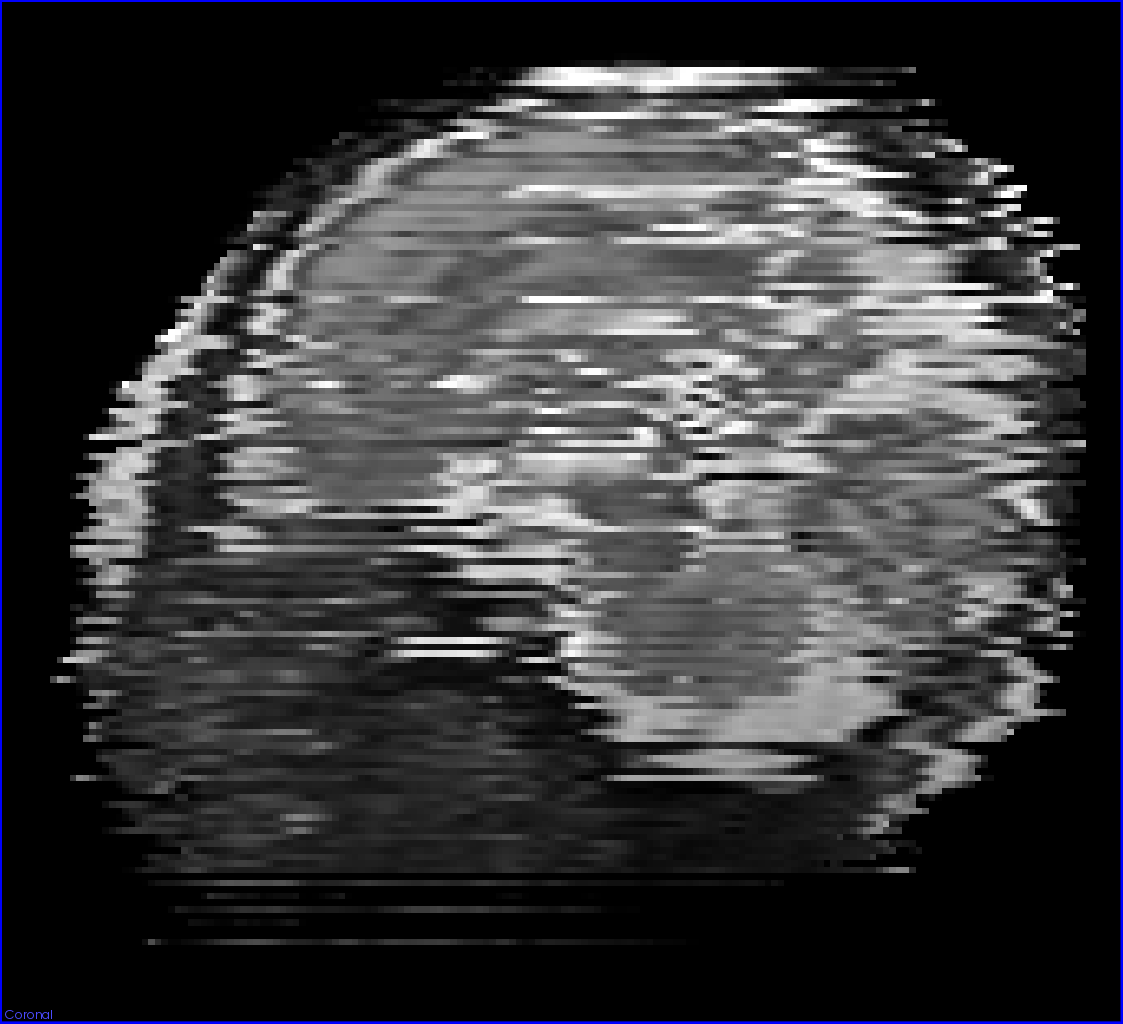
\includegraphics[width=\textwidth]{images/scan_simulation/scan_simulation_10.png}
    \caption{10 Degrees}\label{fig:scan_simulation_10_degrees}
  \end{subfigure}
  ~ %add desired spacing between images, e. g. ~, \quad, \qquad, \hfill etc.
    %(or a blank line to force the subfigure onto a new line)
  \begin{subfigure}[b]{0.32\textwidth}
    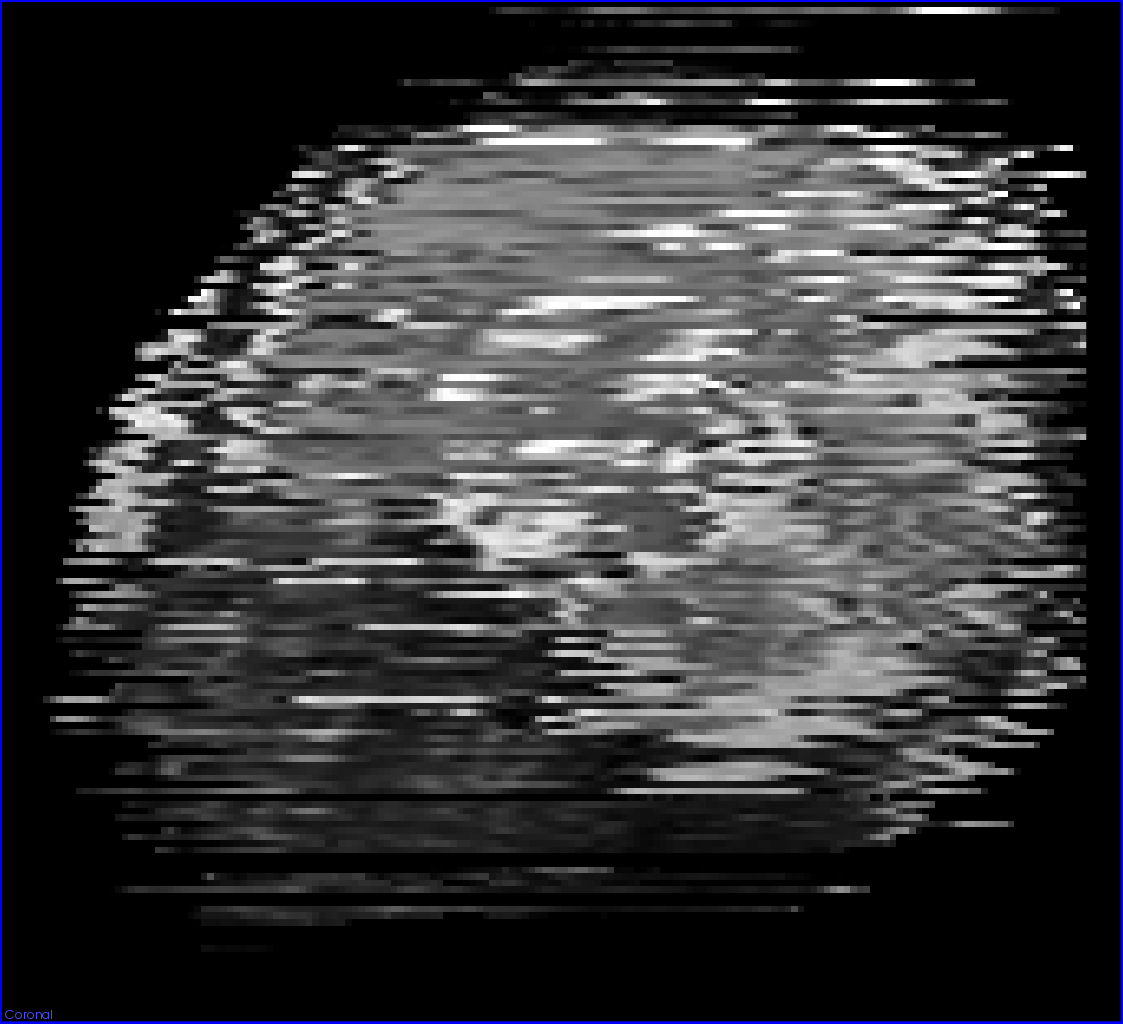
\includegraphics[width=\textwidth]{images/scan_simulation/scan_simulation_20.png}
    \caption{20 Degrees}\label{fig:scan_simulation_20_degrees}
  \end{subfigure}%
  ~ %add desired spacing between images, e. g. ~, \quad, \qquad, \hfill etc.
    %(or a blank line to force the subfigure onto a new line)
  \begin{subfigure}[b]{0.32\textwidth}
    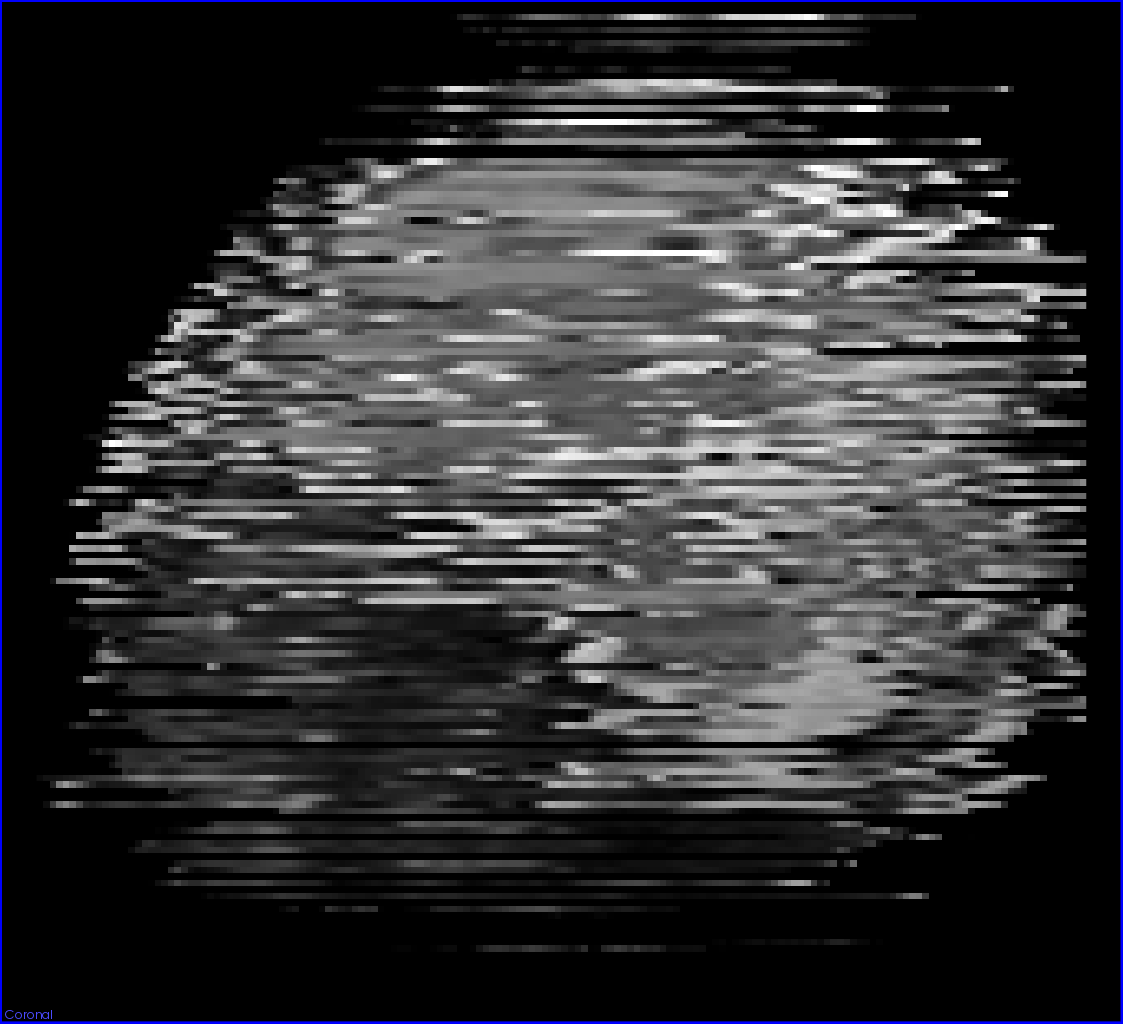
\includegraphics[width=\textwidth]{images/scan_simulation/scan_simulation_30.png}
    \caption{30 Degrees}\label{fig:scan_simulation_30_degrees}
  \end{subfigure}%
  ~ %add desired spacing between images, e. g. ~, \quad, \qquad, \hfill etc.
    %(or a blank line to force the subfigure onto a new line)
  \begin{subfigure}[b]{0.32\textwidth}
    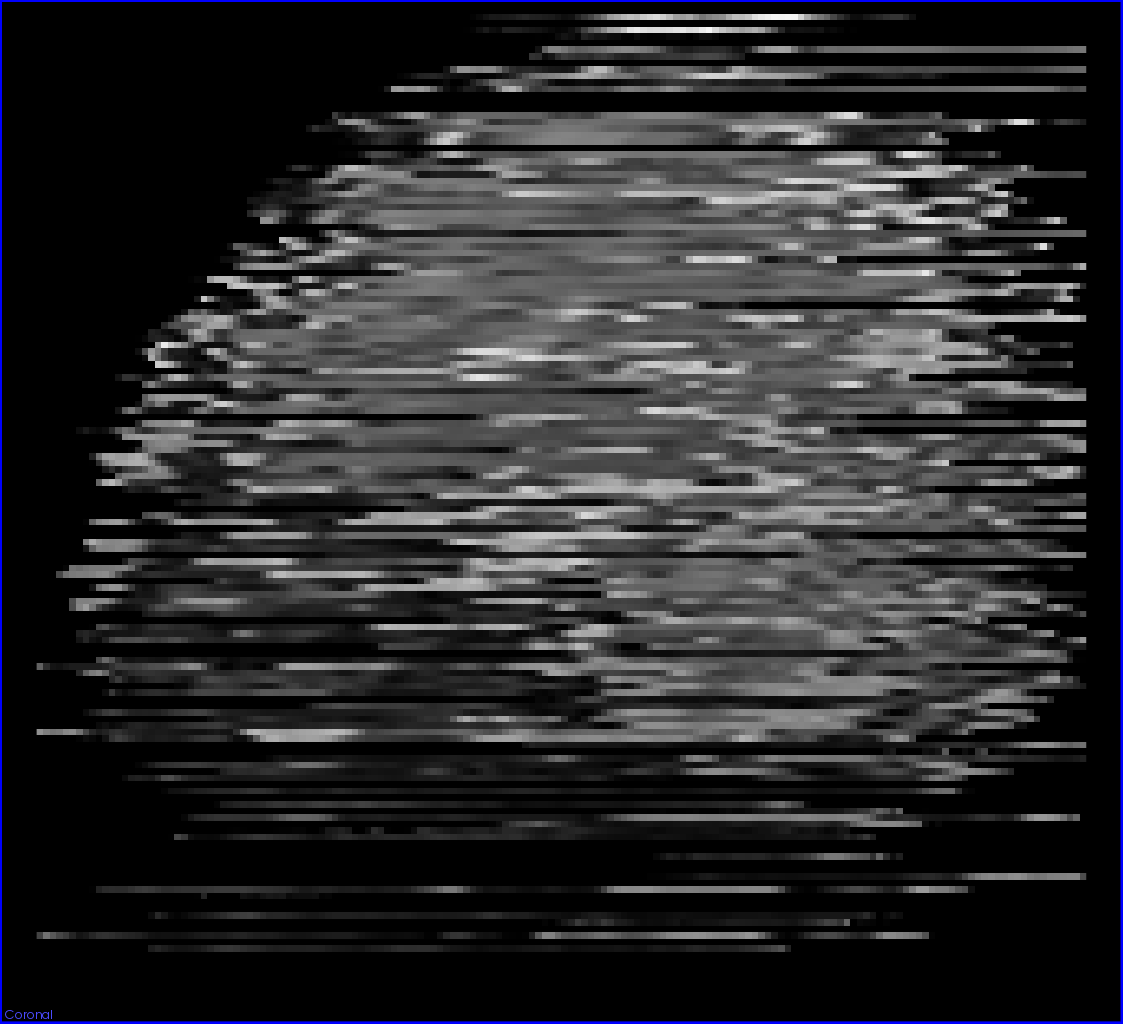
\includegraphics[width=\textwidth]{images/scan_simulation/scan_simulation_45.png}
    \caption{45 Degrees}\label{fig:scan_simulation_45_degrees}
  \end{subfigure}
  \caption{Effects of Motion Corruption}\label{fig:scan_simulation_movement_comparison}
\end{figure}

% ----------------------------- %
% ------- RECONSTRUCTION ------ %
% ----------------------------- %

\clearpage
\section{Reconstruction}\label{method:reconstruction}
This part of the tool provides an interface to the fast GPU reconstruction code developed in \cite{uncertaintysvd}. The implementation makes use of the CTK (Common Toolkit) Command Line Module\cite{ctkcmd}, which allows calls to the GPU code to be made from within the plugin. A wrapper for the code has been written, which conforms to the Command Line Module XML Schema, and this provides the module with all the information it requires to parse the parameters and automatically import the results.

The optional landmarking functionality allows the registration of each of the slices stacks to be guided.

Assuming that the transformation between each of the slice stacks is rigid (translation + rotation) then four points on each stack are needed to perfectly describe the transformation. Figure \ref{fig:rigid_transformation} shows an example 3D object marked up with four points.

\begin{figure}[H]
  \centering
  \begin{subfigure}[b]{0.5\textwidth}
    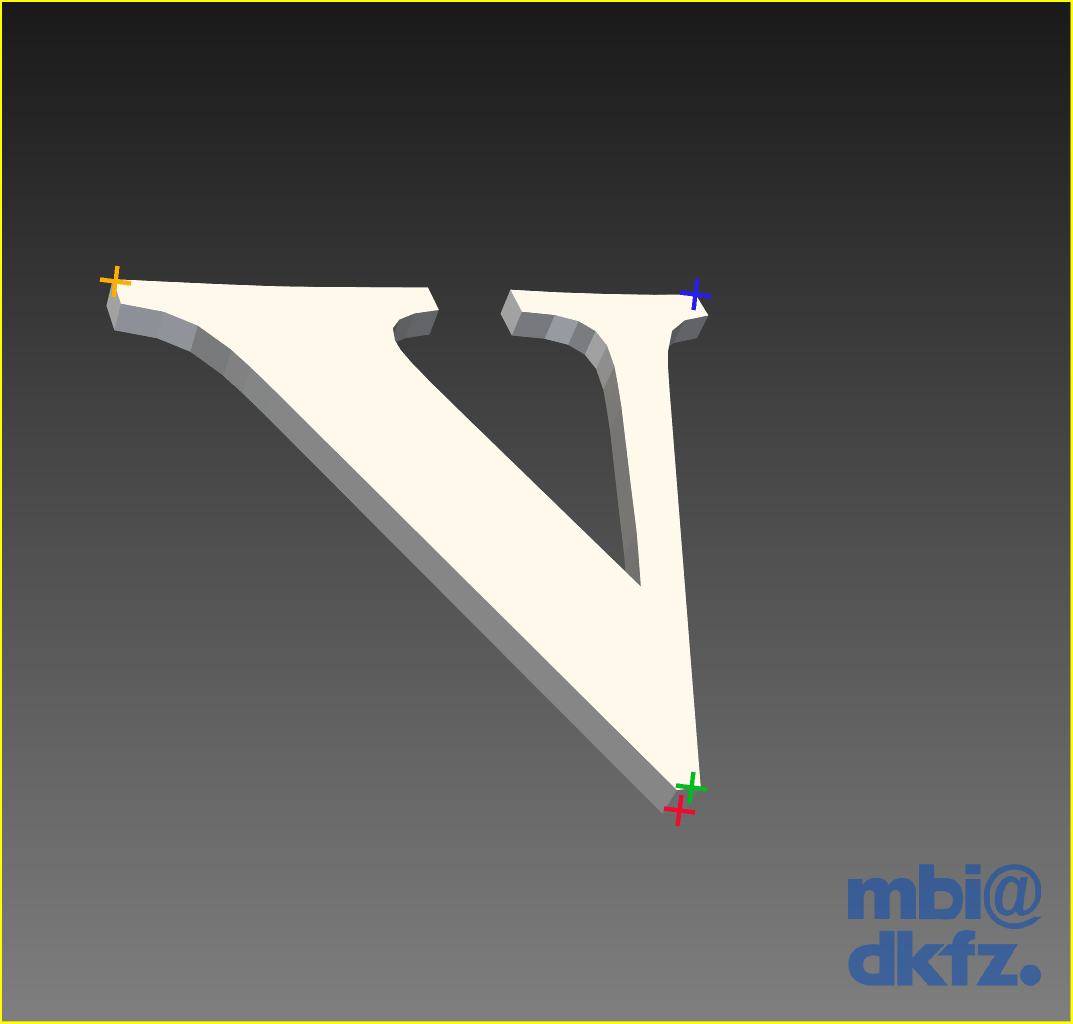
\includegraphics[width=\textwidth]{images/reconstruction/v1.png}
    \caption{Object A}\label{fig:v2}
  \end{subfigure}%
  ~ %add desired spacing between images, e. g. ~, \quad, \qquad, \hfill etc.
    %(or a blank line to force the subfigure onto a new line)
  \begin{subfigure}[b]{0.5\textwidth}
    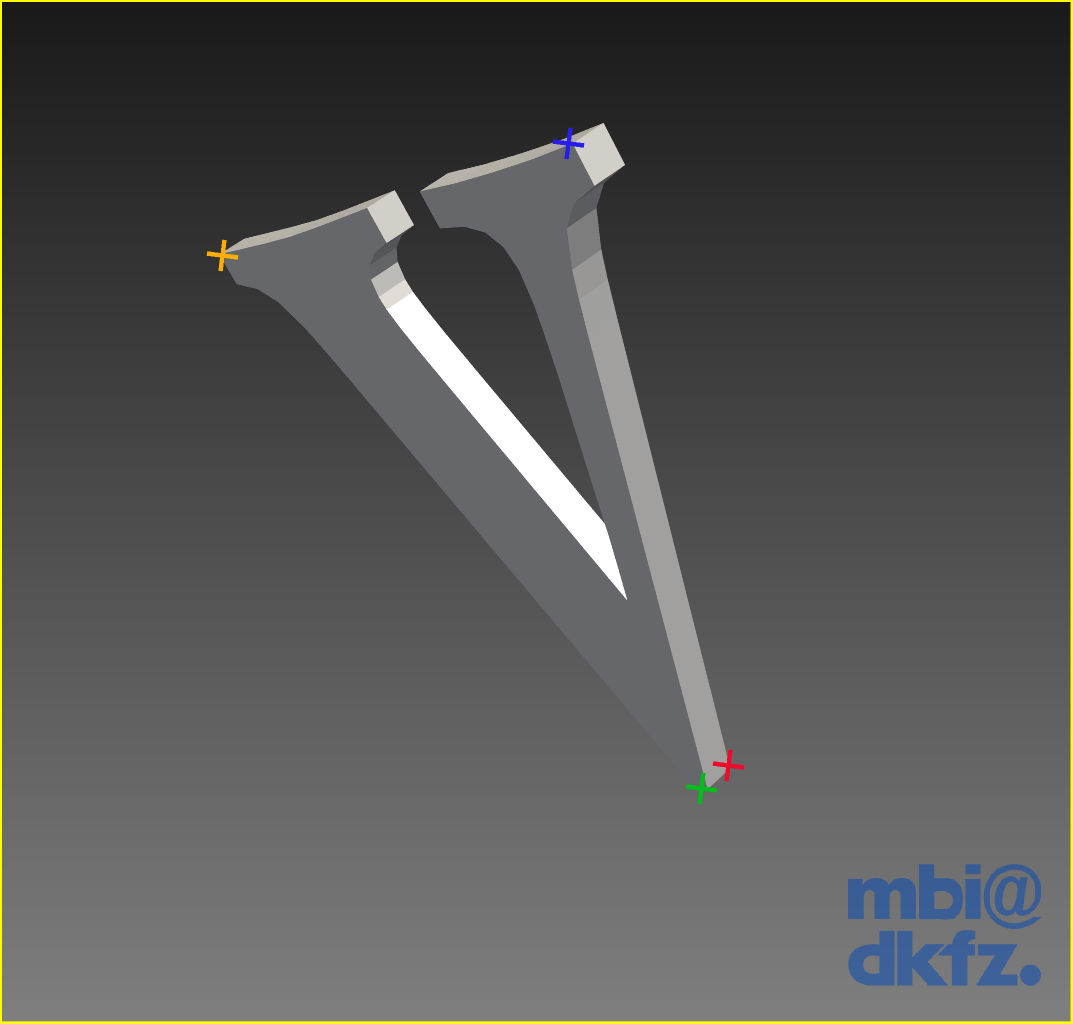
\includegraphics[width=\textwidth]{images/reconstruction/v2.png}
    \caption{Object B}\label{fig:v1}
  \end{subfigure}
  \caption{Example Rigid Transform. Translation + Rotation}\label{fig:rigid_transformation}
\end{figure}

Given only three points the full transformation is ambiguous. Supposing above we did not know the location of the red point in the second object, then there are two possible positions for it, either going away from the camera (relative to the green point) or towards it.

\newpage
The transformation between the two objects can be decided as follows\cite{pointregistration}:

\begin{align*}
          \text{1) Compute axes.} \nonumber \\
          \nonumber \\
  A_x & = A[2] - A[1] \nonumber \\
  A_y & = (A[3] - A[1]) - [(A[3] - O[1]) \cdot A_x]A_x \nonumber \\
  A_z & = +(A_x \times A_y) \text{ if } (A[4] - A[1]) \cdot A_z > 0\nonumber \\  
  A_z & = -(A_x \times A_y) \text{ if } (A[4] - A[1]) \cdot A_z < 0\nonumber \\
          \nonumber \\
          \text{...and the same for B.} \nonumber \\
          \nonumber \\
  \text{where}& \\
  & X[p] \text{ - point $p$ in object $X$} \nonumber \\
  & X_x \text{ - x axis of object $X$} \nonumber \\
  & X_y \text{ - y axis of object $X$} \nonumber \\
  & X_z \text{ - z axis of object $X$} \nonumber \\
          \nonumber \\
          \text{2) Build rotation matrices.} \nonumber \\
          \nonumber \\
  R_A & = [A_x; A_y; A_z] \nonumber \\
  R_B & = [B_x; B_y; B_z] \nonumber \\
          \nonumber \\
          \text{3) Rotation, $R$, from $A$ to $B$:} \nonumber \\
          \nonumber \\
  R R_A & = R_B \nonumber \\
  R & = R_B R_A^{-1} \nonumber \\
  R & = R_B R_A^T \text{ ($R^{-1} = R^T$ for rotation matrices)} \nonumber \\
          \nonumber \\
          \text{4) Translation, $T$, from $A$ to $B$:} \nonumber \\
          \nonumber \\
  T & = B[1] - R A[1] \nonumber \\     
\end{align*}

% ----------------------------- %
% ------- VISUALIZATIONS ------ %
% ----------------------------- %

\clearpage
\section{Visualizations}

% ------------------------- %
% ------ UNCERTAINTY ------ %
% ------------------------- %
\subsection{Uncertainty}\label{method:uncertainty}
Three different types of uncertainty have been considered, though with different reconstruction algorithms there may be other metrics that can be extracted.

\begin{enumerate}
  \item sampling - How many points in the original scans correspond to the area in the reconstruction? Some parts of reconstruction will have many points in the original stacks to use, but others will not more interpolation will be required.
  \item registration - How precisely is the registration known? Depending on the calibration of the scanner and the amount of movement that occurs during the scan our confidence in the registration will change.
  \item intensity bias - Bias is an artefact that occurs in MRI that means that some areas of the image are darker than others, not due to the tissue itself, but the distance from the receiver coil. Some areas have more of this inhomogeneity than others and contrast will be affected.
\end{enumerate}

Having three separate 'channels' of uncertainty makes visualizing it more difficult. Trying to display all three at one time will likely be too much information to communicate at once however all of the visualizations developed are applicable to each individually or alternately the three types can be aggregated into one combined value.

An aggregation of all three will be able to give a useful overview of the situation, however being able to isolate a single type of uncertainty is important as it gives the viewer an idea of what caused the reconstruction issues.

% ----------------------------- %
% ------- PRE-PROCESSING ------ %
% ----------------------------- %

\subsection{Pre-processing}\label{method:pre-processing}
Before the uncertainty is visualized it is first pre-processed. Figure \ref{fig:preprocesspipeline} illustrates the order in which the operations are applied. Operations with a dotted border are optional.

\begin{figure}[H]
  \centering
  
\includegraphics[width=0.8\textwidth]{images/pre-process_pipeline.png}
  \caption{Pre-processing pipeline overview.}
  \label{fig:preprocesspipeline}
\end{figure}

\subsubsection*{Normalize}
The uncertainty is linearly scaled so each value lies between 0 (bad) and 1 (good).

\subsubsection*{Invert}
The uncertainty can be inverted if saved the opposite way around.\\(\texttt{Uncertainty = 1 - Uncertainty})

\subsubsection*{Erosion}
The edges of the uncertainty are removed in three steps:

\begin{enumerate}
  \item The image is thresholded to create a mask of the background.
  \item The mask is then expanded using binary morphology.
  \item Then all the points in the mask are set to 0 (background) to remove the edge.
\end{enumerate}

Figure \ref{fig:erosionoverview} shows how the soft fade out of uncertainty due to the mask is removed to create a hard edge.

\begin{figure}[h]
  \centering
  \begin{subfigure}[b]{0.45\textwidth}
    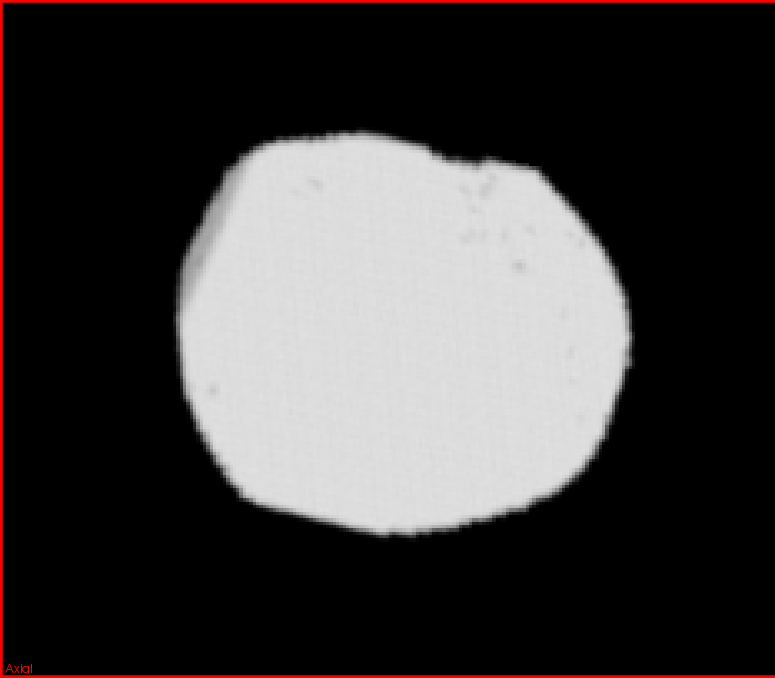
\includegraphics[width=\textwidth]{images/erosion/erosion_0.png}
    \caption{Original}
    \label{fig:erosion0}
  \end{subfigure}%
  ~ %add desired spacing between images, e. g. ~, \quad, \qquad, \hfill etc.
    %(or a blank line to force the subfigure onto a new line)
  \begin{subfigure}[b]{0.45\textwidth}
    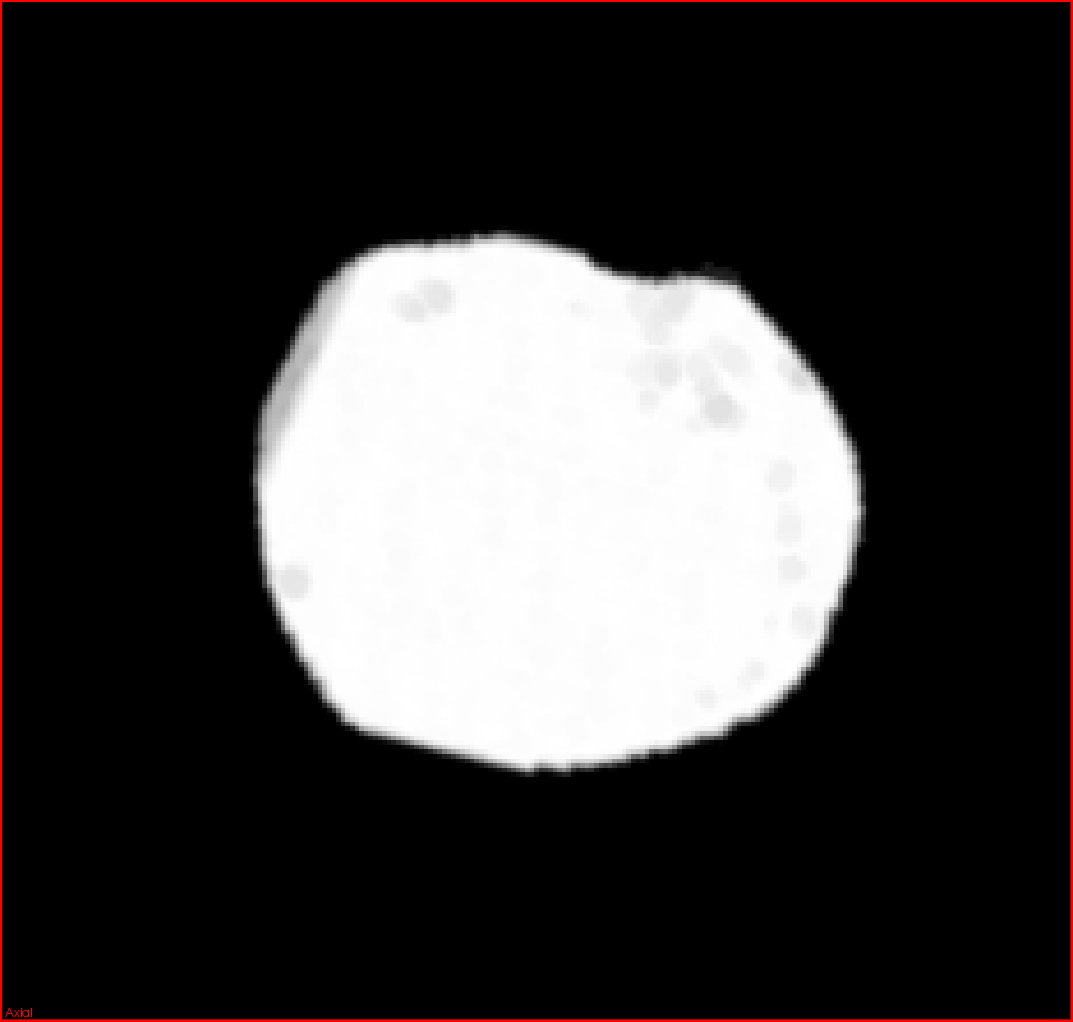
\includegraphics[width=\textwidth]{images/erosion/erosion_1.png}
    \caption{Step 1}
    \label{fig:erosion1}
  \end{subfigure}  
  ~ %add desired spacing between images, e. g. ~, \quad, \qquad, \hfill etc.
    %(or a blank line to force the subfigure onto a new line)
  \begin{subfigure}[b]{0.45\textwidth}
    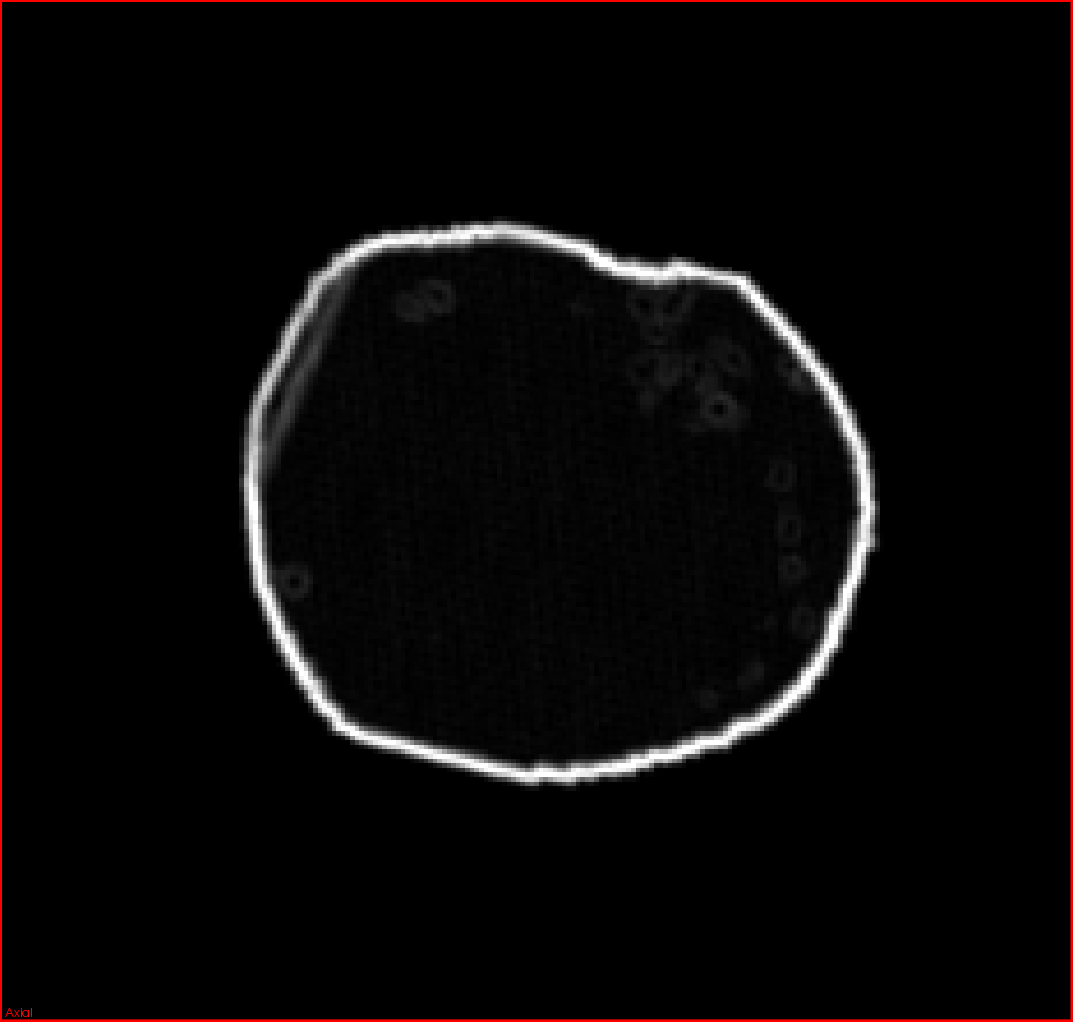
\includegraphics[width=\textwidth]{images/erosion/erosion_2.png}
    \caption{Step 2}
    \label{fig:erosion2}
  \end{subfigure}%
  ~ %add desired spacing between images, e. g. ~, \quad, \qquad, \hfill etc.
    %(or a blank line to force the subfigure onto a new line)
  \begin{subfigure}[b]{0.45\textwidth}
    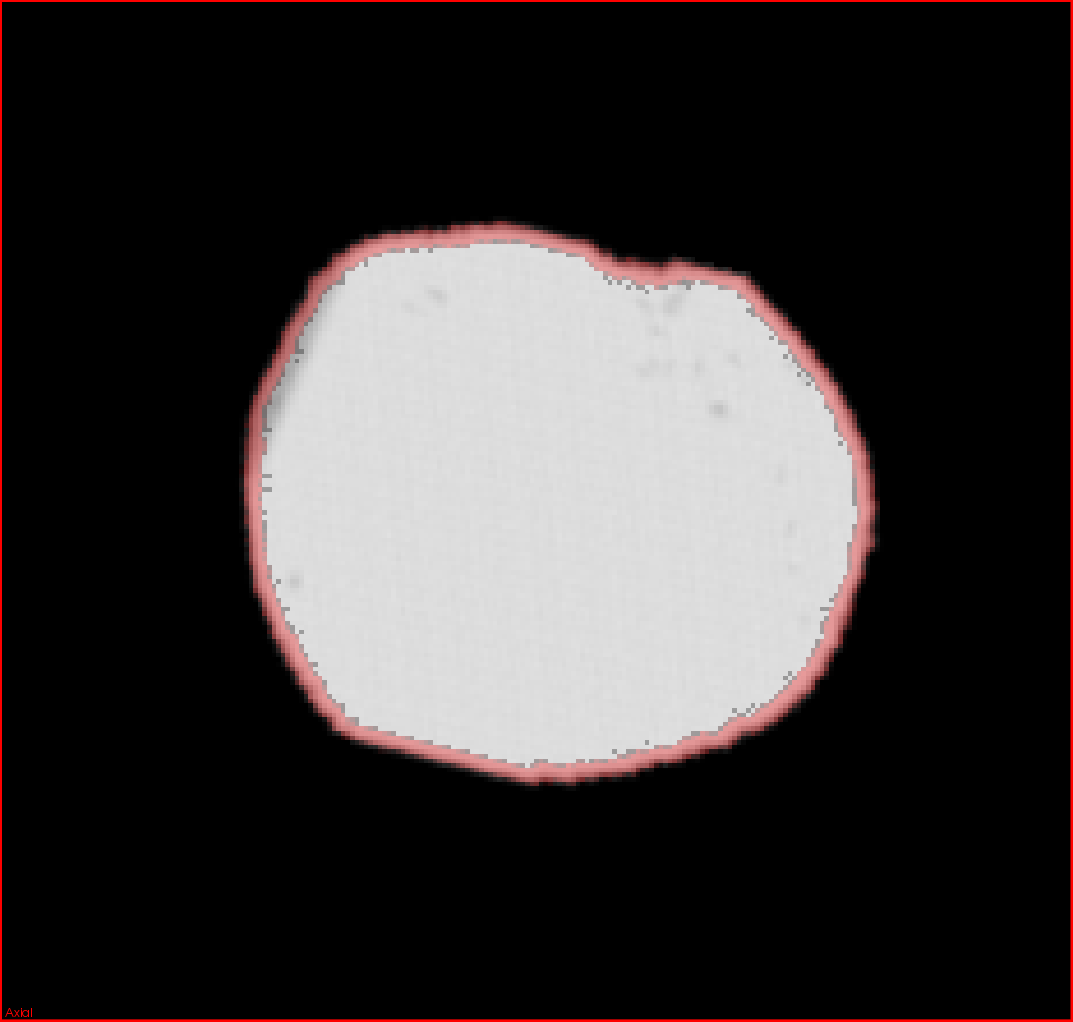
\includegraphics[width=\textwidth]{images/erosion/erosion_3.png}
    \caption{Result}
    \label{fig:erosion3}
  \end{subfigure}  
  \caption{Steps involved in removing the edge.}\label{fig:erosionoverview}
\end{figure}

Figure \ref{fig:growing} explains how the binary morphology in step 2 works. Each value in the image is either in the mask or out of the mask. To grow the mask a neighbourhood around each point is examined and if any neighbour is in the mask then that point is added to the mask. The size and shape of the neighbourhood determines how much the mask grows.

\begin{figure}[H]
  \centering
  \begin{subfigure}[b]{0.5\textwidth}
    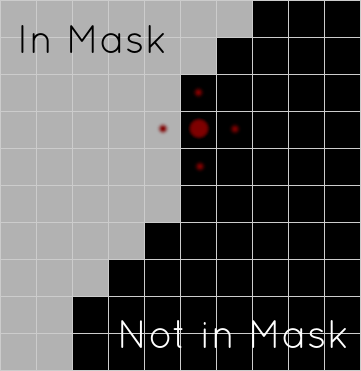
\includegraphics[width=\textwidth]{images/erosion/growing_1.png}
    \caption{An example neighbourhood.}\label{fig:growing_1}
  \end{subfigure}%
  ~ %add desired spacing between images, e. g. ~, \quad, \qquad, \hfill etc.
    %(or a blank line to force the subfigure onto a new line)
  \begin{subfigure}[b]{0.5\textwidth}
    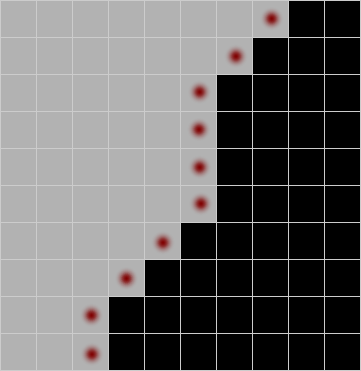
\includegraphics[width=\textwidth]{images/erosion/growing_2.png}
    \caption{The mask grows.}\label{fig:growing_2}
  \end{subfigure}
  \caption{Example of binary morphology.}\label{fig:growing}
\end{figure}

\subsubsection*{Align to Scan}
The image to world matrix of the scan is copied to the uncertainty volume. This results in pixel (x, y, z) in both the scan and uncertainty being mapped to the same point in space, allowing one to be overlayed on the other.

% ------------------------------- %
% ------- TEST UNCERTAINTY ------ %
% ------------------------------- %

\clearpage
\subsection{Test Uncertainties}\label{method:test_uncertainties}
To test and debug each visualization a number of artificial uncertainties have been created as well as an example from a genuine fetal brain reconstruction.

\subsubsection*{Sphere of Uncertainty}
An uncertainty volume where the uncertainty is proportional to the distance from the center. The uncertainty is 0 (very bad) at the center and 1 (very good) at the edges.

\subsubsection*{Sphere in Corner}
Similar to the sphere, but instead of being placed in the middle it is placed in one corner of the volume.

\subsubsection*{Cube of Uncertainty}
An uncertainty volume that is 1 (very good) everywhere except for fixed size cube of uncertainty 0 (very bad) in the center.

\subsubsection*{Random Uncertainty}
The uncertainty at every point is a random uniformly distributed value.

\subsubsection*{Reconstruction Uncertainty}
Uncertainty generated from an example super-resolution reconstruction of a fetal brain.\\

\begin{figure}[h]
  \centering
  \begin{subfigure}[b]{0.18\textwidth}
    \fcolorbox{gray}{white}{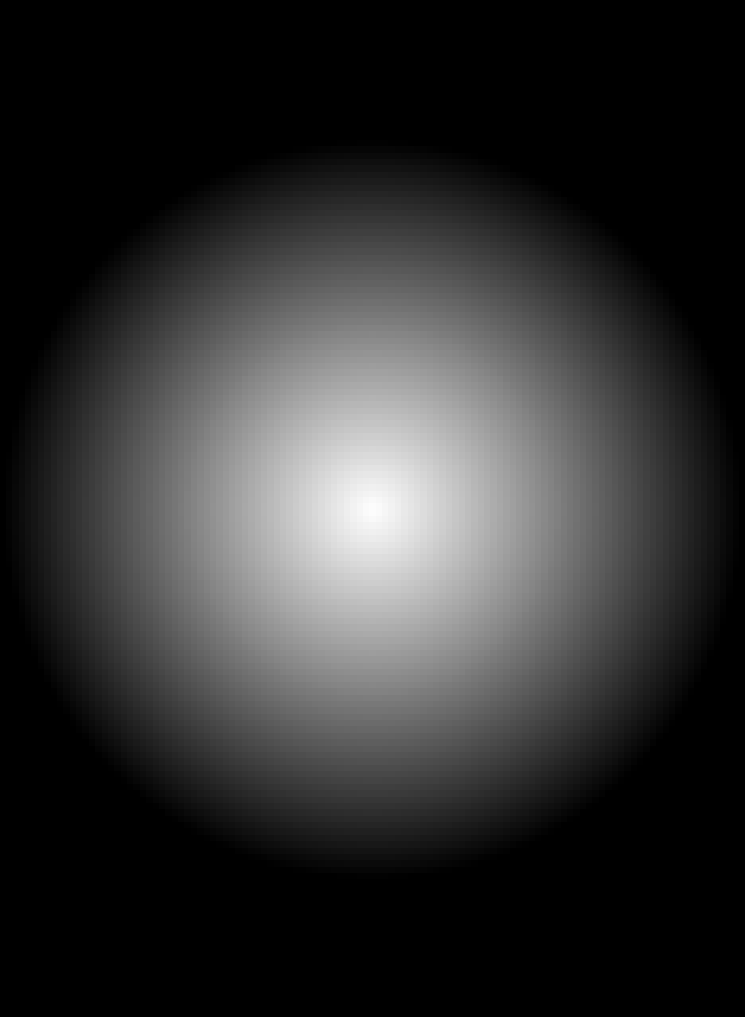
\includegraphics[width=\textwidth]{images/test/test_sphere.png}}
    \caption{Sphere}
    \label{fig:test_sphere}
  \end{subfigure}%
  ~~%add desired spacing between images, e. g. ~, \quad, \qquad, \hfill etc.
    %(or a blank line to force the subfigure onto a new line)
  \begin{subfigure}[b]{0.18\textwidth}
    \fcolorbox{gray}{white}{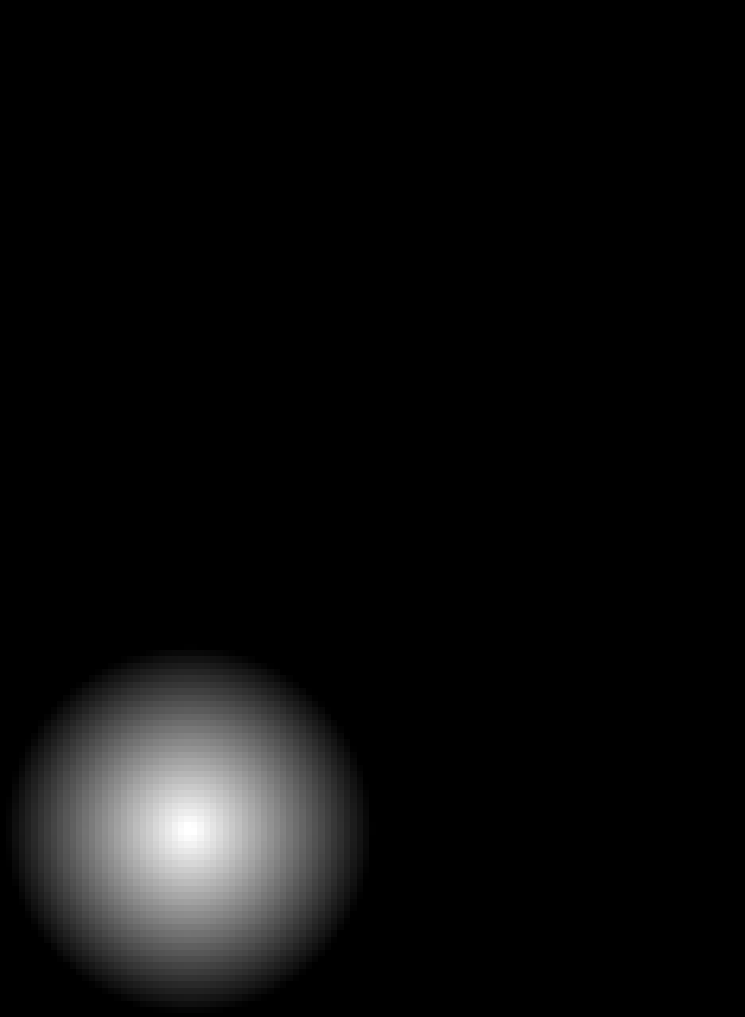
\includegraphics[width=\textwidth]{images/test/test_quadsphere.png}}
    \caption{Corner}
    \label{fig:test_corner}
  \end{subfigure}%
  ~~%add desired spacing between images, e. g. ~, \quad, \qquad, \hfill etc.
    %(or a blank line to force the subfigure onto a new line)
  \begin{subfigure}[b]{0.18\textwidth}
    \fcolorbox{gray}{white}{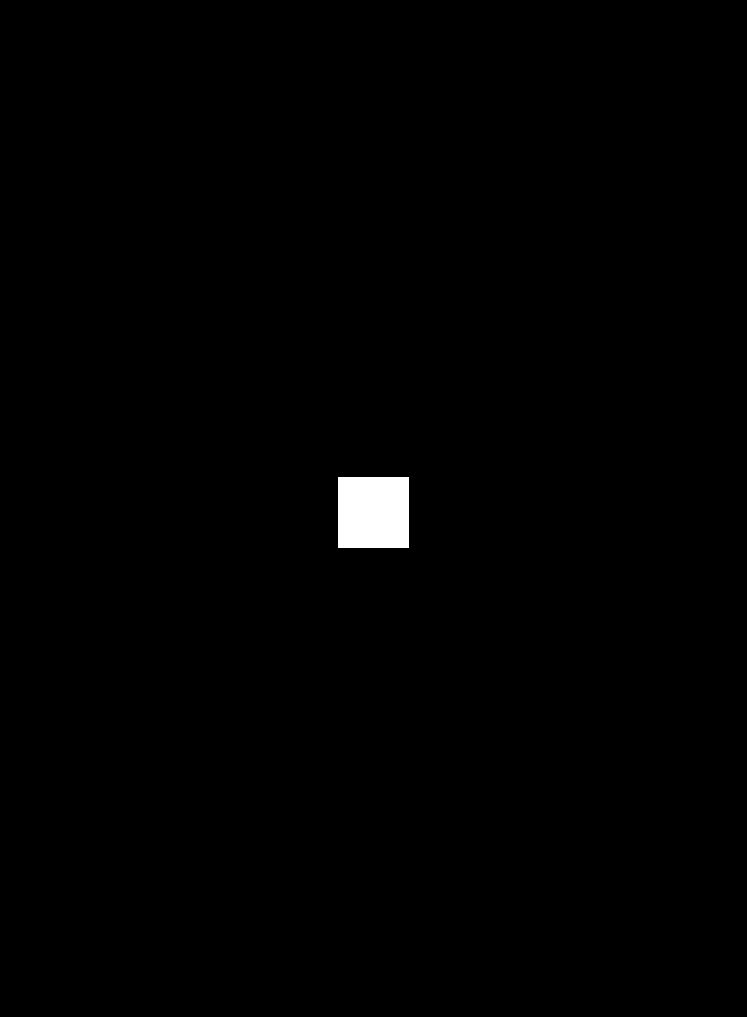
\includegraphics[width=\textwidth]{images/test/test_cube.png}}
    \caption{Cube}
    \label{fig:test_cube}
  \end{subfigure}%
  ~~%add desired spacing between images, e. g. ~, \quad, \qquad, \hfill etc.
    %(or a blank line to force the subfigure onto a new line)
  \begin{subfigure}[b]{0.18\textwidth}
    \fcolorbox{gray}{white}{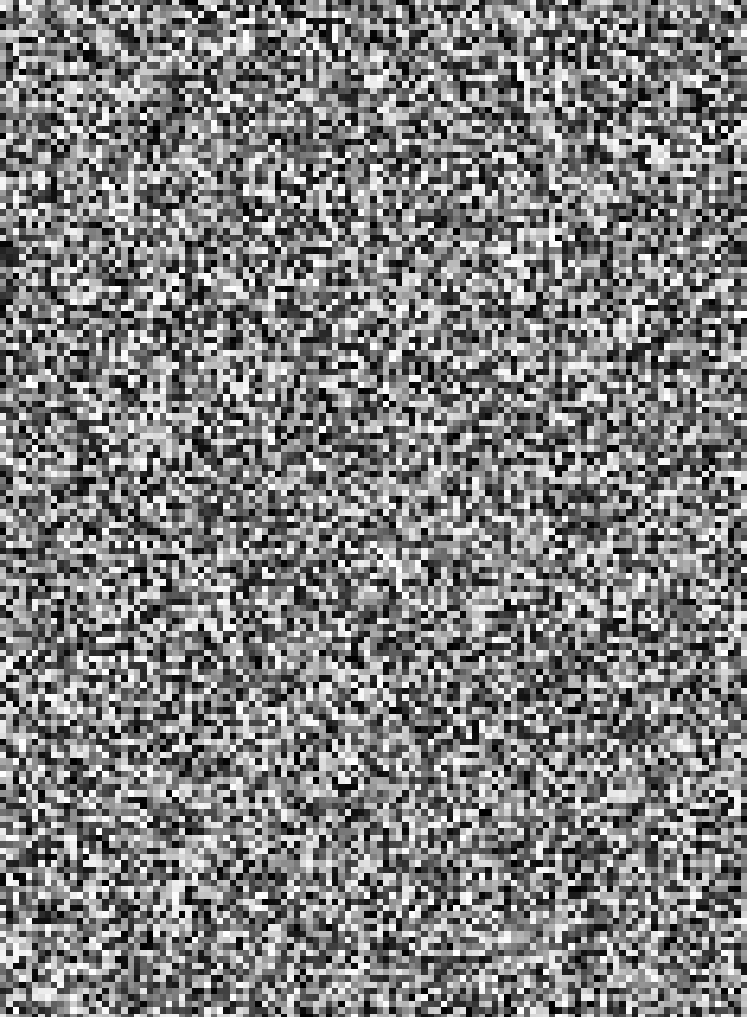
\includegraphics[width=\textwidth]{images/test/test_random.png}}
    \caption{Random}
    \label{fig:test_random}
  \end{subfigure}%
  ~~%add desired spacing between images, e. g. ~, \quad, \qquad, \hfill etc.
    %(or a blank line to force the subfigure onto a new line)
  \begin{subfigure}[b]{0.18\textwidth}
    \fcolorbox{gray}{white}{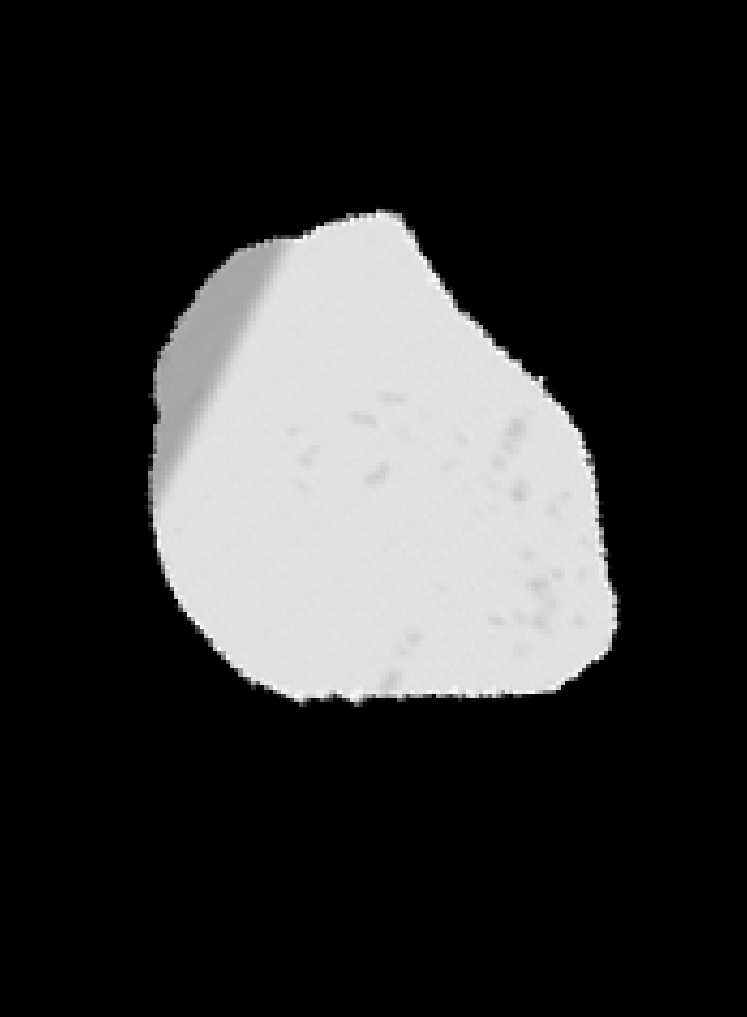
\includegraphics[width=\textwidth]{images/test/test_scan.png}}
    \caption{Fetal Brain}
    \label{fig:test_example}
  \end{subfigure}
  \caption{Test Uncertainty Volumes.}\label{fig:test_uncertainties}
\end{figure}

% ----------------------------- %
% -------- THRESHOLDING ------- %
% ----------------------------- %

\clearpage
\subsection{Thresholding}\label{method:thresholding}
The idea behind thresholding is to isolate areas in the reconstructed image that are within a particular range of uncertainty. This visualization can be viewed in both 2D and 3D.

The visualization is realised by first creating a binary mask, set to 1 where the uncertainty is within the range [min, max] and 0 where it is not. This mask can then be rendered transparently on top of the reconstructed scan in 2D so both the uncertain area and underlying scan can be seen simultaneously. See figure \ref{fig:thresholding2d}.

\begin{figure}[H]
  \centering
  \begin{subfigure}[b]{0.3\textwidth}
    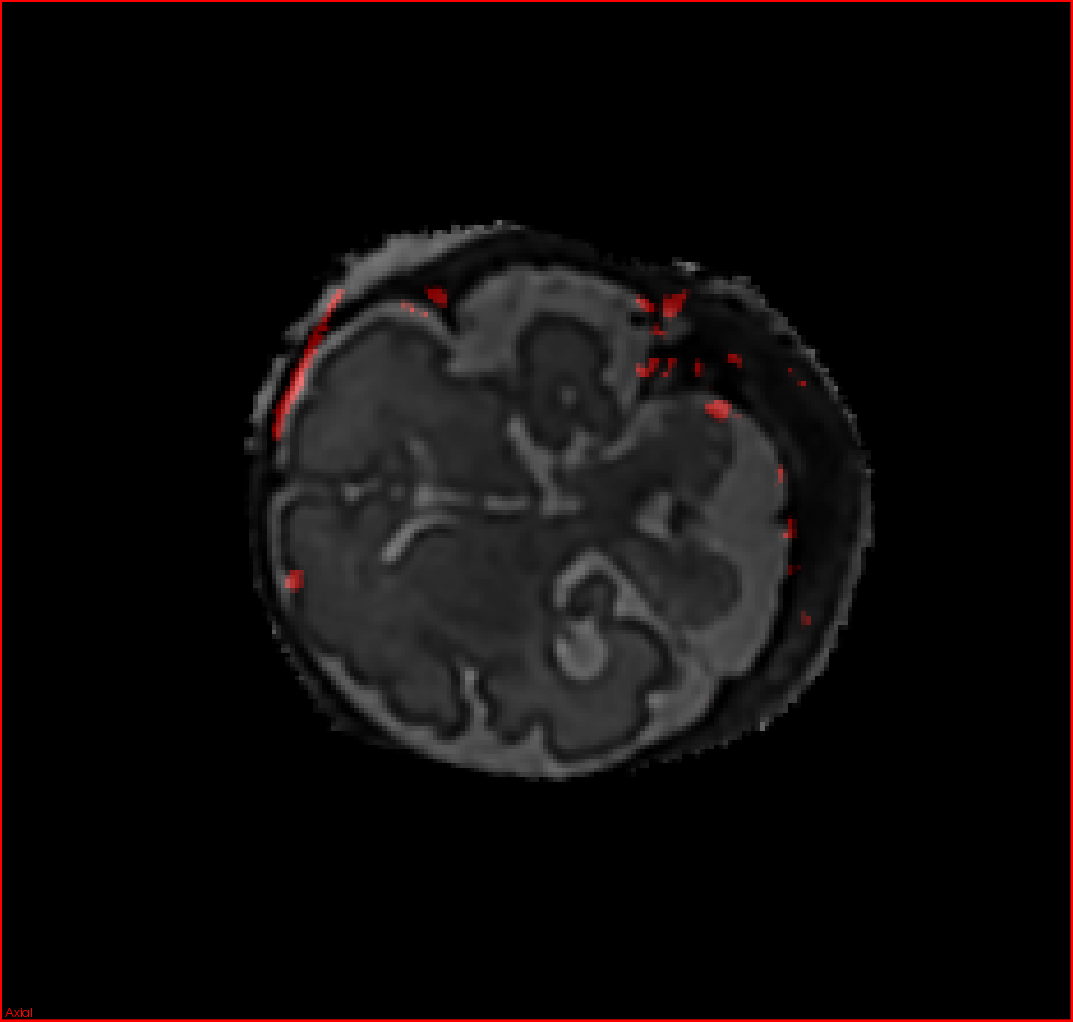
\includegraphics[width=\textwidth]{images/thresholding/thresholding_2d_axial.png}
    \caption{Axial}
    \label{fig:thresholding2daxial}
  \end{subfigure}%
  ~ %add desired spacing between images, e. g. ~, \quad, \qquad, \hfill etc.
    %(or a blank line to force the subfigure onto a new line)
  \begin{subfigure}[b]{0.3\textwidth}
    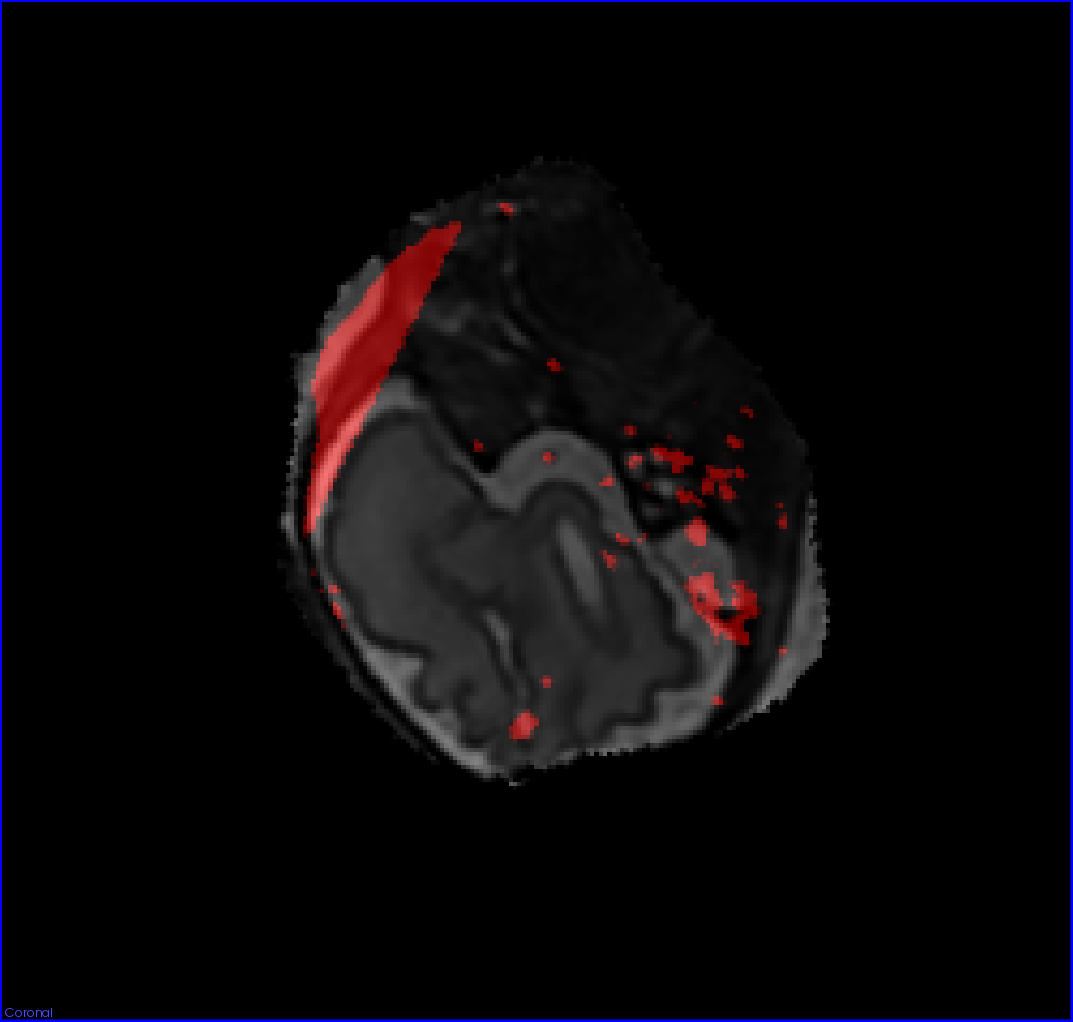
\includegraphics[width=\textwidth]{images/thresholding/thresholding_2d_coronal.png}
    \caption{Coronal}
    \label{fig:thresholding2dcoronal}
  \end{subfigure}%
  ~ %add desired spacing between images, e. g. ~, \quad, \qquad, \hfill etc.
    %(or a blank line to force the subfigure onto a new line)
  \begin{subfigure}[b]{0.3\textwidth}
    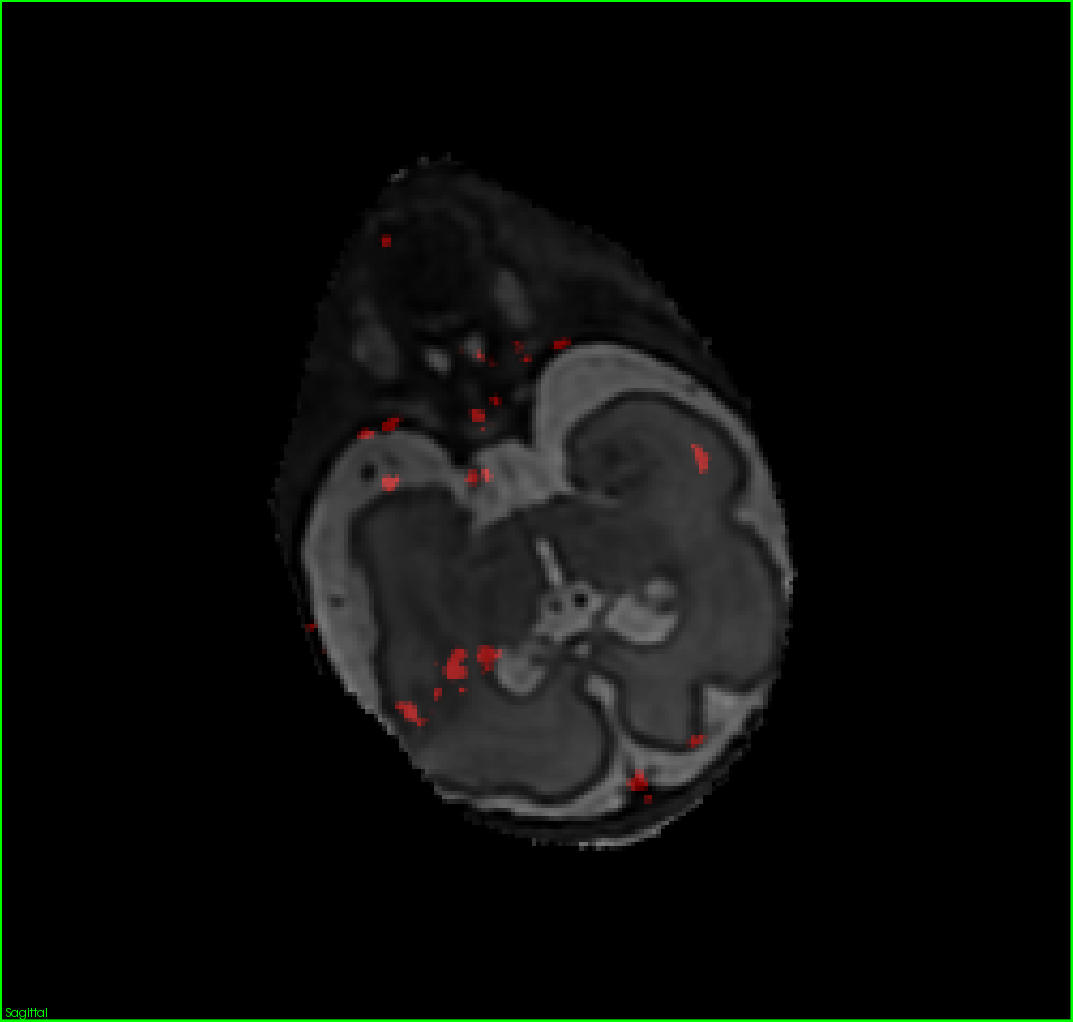
\includegraphics[width=\textwidth]{images/thresholding/thresholding_2d_sagittal.png}
    \caption{Sagittal}
    \label{fig:thresholding2dsagittal}  
  \end{subfigure}
  \caption{Thresholding in 2D}\label{fig:thresholding2d}
\end{figure}

To view the uncertainty in 3D, two variations have been implemented, both using volume rendering (see section \ref{background:volumerendering}). Variation 1 applies volume rendering directly to the uncertainty and variation 2 applies volume rendering to the binary mask.

The transfer functions used in each variation can be seen in figure \ref{fig:thresholdingoverview}. The first works by making values within the thresholded range opaque and those outside it transparent. The second works in a similar way; 0 in the mask is out of the range and 1 in the mask is in the range. In the second transfer function there is a slow fade out, rather than a sharp change, to give individual points of uncertainty some presence.

\begin{figure}[H]
  \centering
  \begin{subfigure}[b]{0.5\textwidth}
    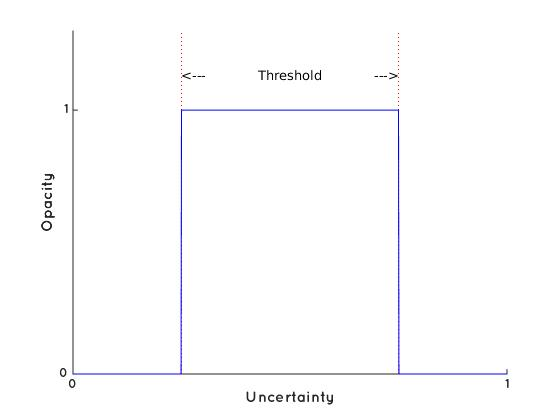
\includegraphics[width=\textwidth]{images/thresholding/thresholdvariation1.jpg}
    \caption{Variation 1}
    \label{fig:thresholdingvariation1}
  \end{subfigure}%
  ~ %add desired spacing between images, e. g. ~, \quad, \qquad, \hfill etc.
    %(or a blank line to force the subfigure onto a new line)
  \begin{subfigure}[b]{0.5\textwidth}
    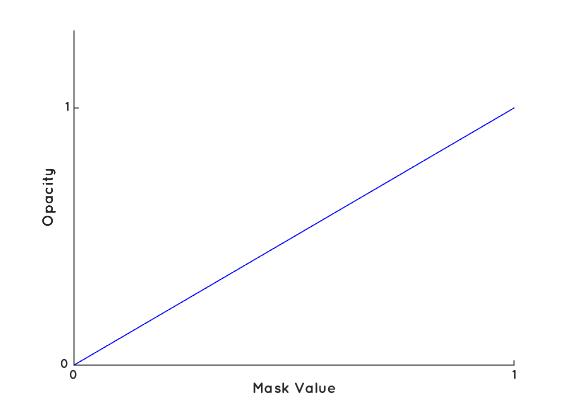
\includegraphics[width=\textwidth]{images/thresholding/thresholdvariation2.jpg}
    \caption{Variation 2}
    \label{fig:thresholdingvariation2}
  \end{subfigure}
  \caption{Opacity Transfer Functions. Opacity of 0 is transparent, 1 is opaque.}\label{fig:thresholdingoverview}
\end{figure}

An issue found with variation 1 was that the renderer still draws the edge of the uncertainty, even though it had previously been removed by erosion. This is due to the renderer using linear interpolation to take samples along each ray fired into the volume. Figure \ref{fig:thresholdingvariation1problem} illustrates the problem: the background has uncertainty 0.0, and the object has uncertainty $\sim$0.6. Points interpolated between the two will lie in the range [0.0-0.6] and so we find values of uncertainty that don't actually exist in the object.

\begin{figure}[h]
  \centering
  \begin{subfigure}[b]{0.481\textwidth}
    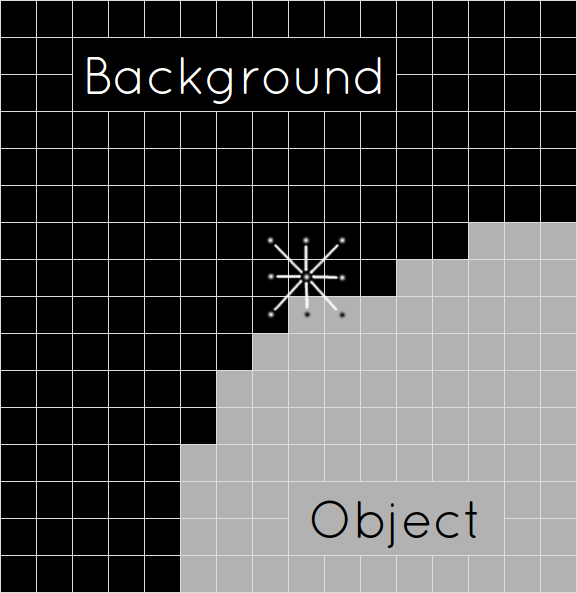
\includegraphics[width=\textwidth]{images/thresholding/thresholdvariation1example.png}
    \caption{Simplified View}
    \label{fig:thresholdingvariation1example}
  \end{subfigure}%
  ~ %add desired spacing between images, e. g. ~, \quad, \qquad, \hfill etc.
    %(or a blank line to force the subfigure onto a new line)
  \begin{subfigure}[b]{0.519\textwidth}
    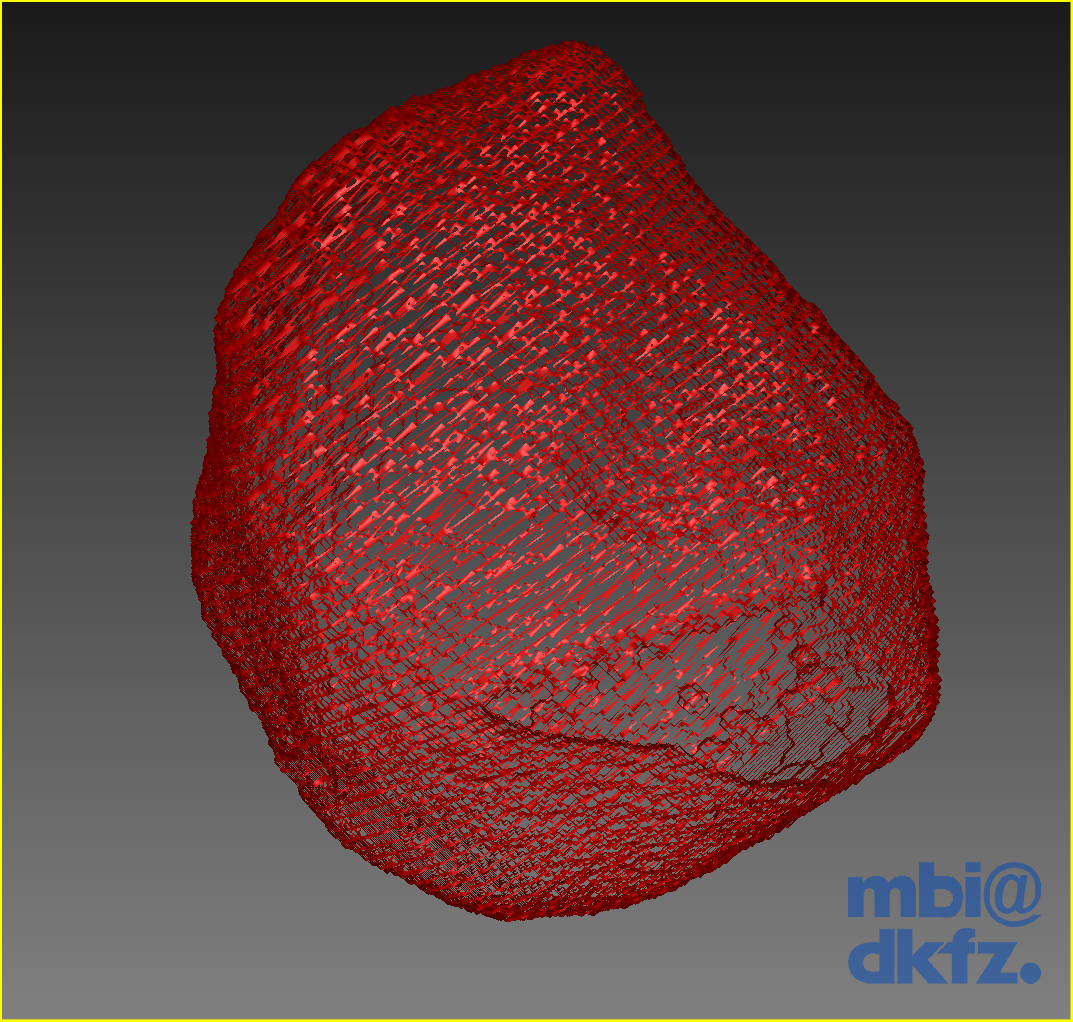
\includegraphics[width=\textwidth]{images/thresholding/thresholdvariation1problem.png}
    \caption{Edge Artefacts}
    \label{fig:thresholdingvariation1artefacts}
  \end{subfigure}
  \caption{Edge artefacts.}\label{fig:thresholdingvariation1problem}
\end{figure}

A solution to this problem is to use a gradient transfer function which allows the change in uncertainty to influence the transparency. Rapid changes in uncertainty can therefore be treated as noise and ignored. The cutoff can be adjusted to remove the entire edge but there is a tradeoff as some genuine regions of uncertainty can also be filtered out. Figure \ref{fig:thresholdingvariationfix} shows the transfer function and the effect of tweaking the threshold.

\begin{figure}[H]
  \centering
  \begin{subfigure}[b]{0.5\textwidth}
    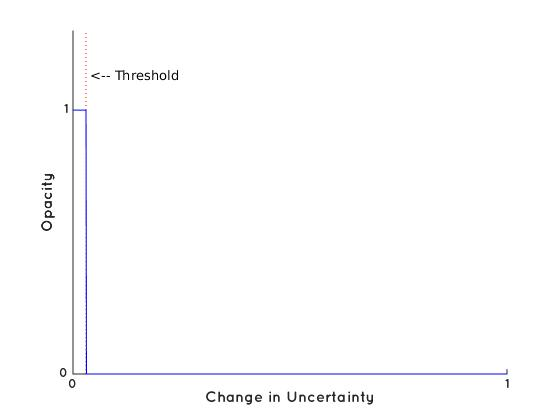
\includegraphics[width=\textwidth]{images/thresholding/thresholdvariation1fix.jpg}
    \caption{Gradient Transfer Function}
    \label{fig:thresholdvariation1fix}
  \end{subfigure}%
  ~ %add desired spacing between images, e. g. ~, \quad, \qquad, \hfill etc.
    %(or a blank line to force the subfigure onto a new line)
  \begin{subfigure}[b]{0.5\textwidth}
    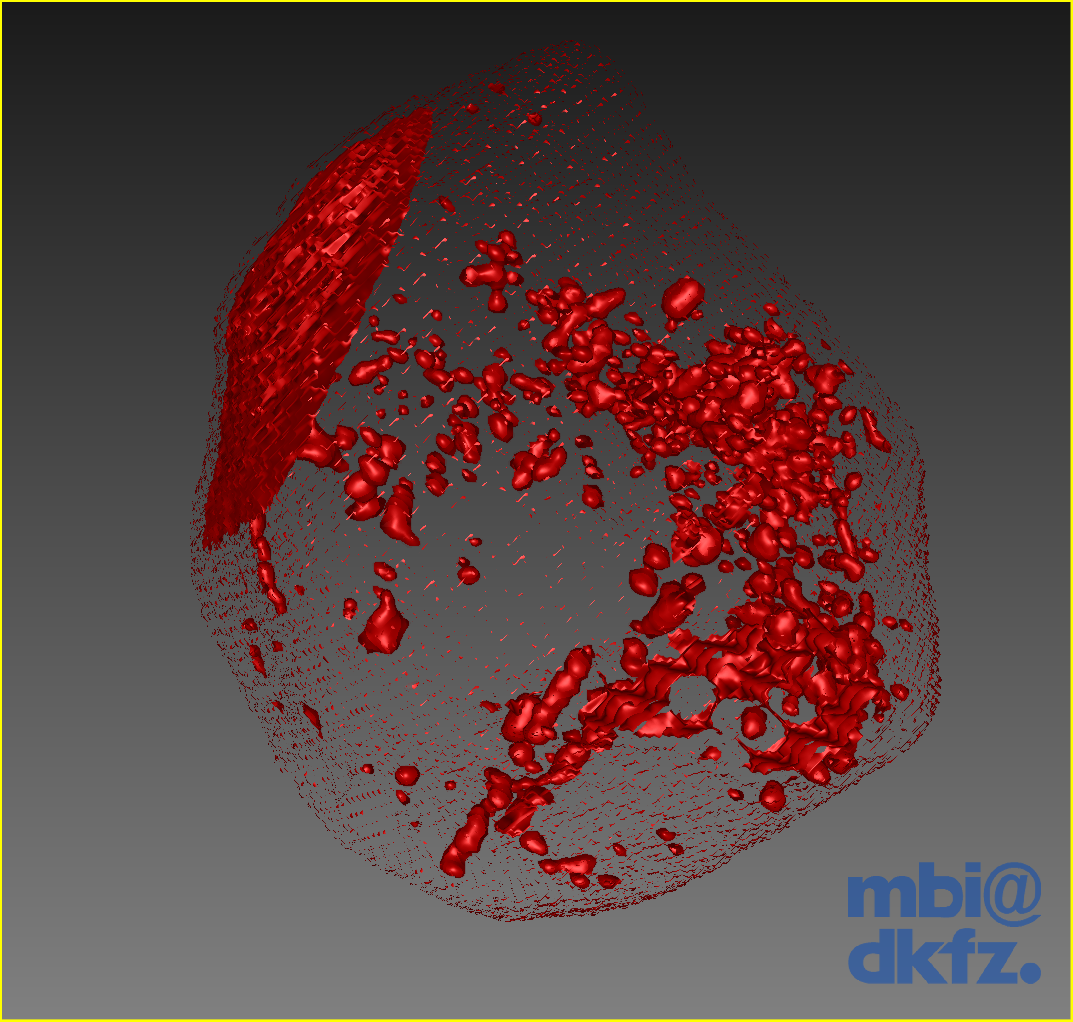
\includegraphics[width=\textwidth]{images/thresholding/thresholdvariation1threshold1.png}
    \caption{Threshold 0.05}
    \label{fig:thresholdingvariation1threshold1}
  \end{subfigure}\\[11pt]
  \begin{subfigure}[b]{0.5\textwidth}
    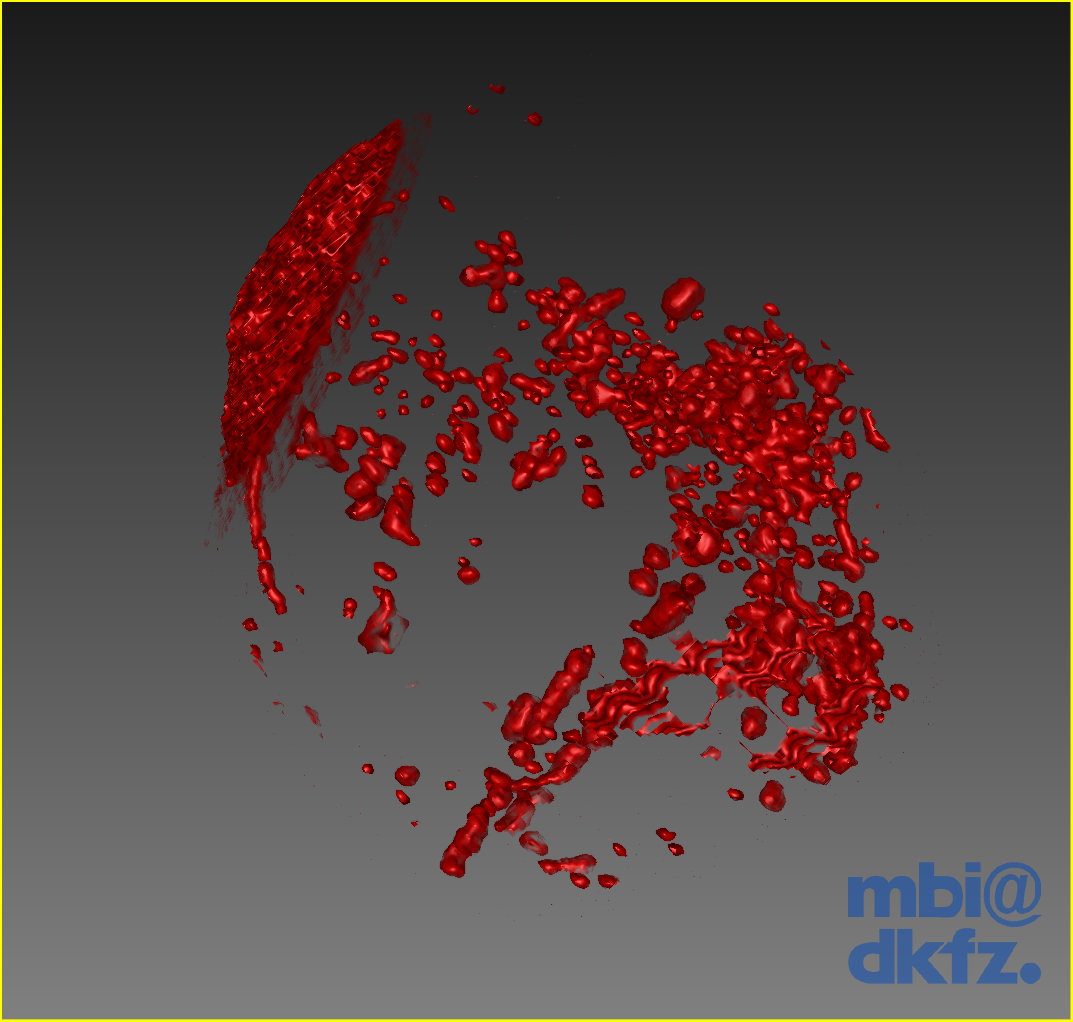
\includegraphics[width=\textwidth]{images/thresholding/thresholdvariation1threshold2.png}
    \caption{Threshold 0.02}
    \label{fig:thresholdingvariation1threshold2}  
  \end{subfigure}%
  ~ %add desired spacing between images, e. g. ~, \quad, \qquad, \hfill etc.
    %(or a blank line to force the subfigure onto a new line)
  \begin{subfigure}[b]{0.5\textwidth}
    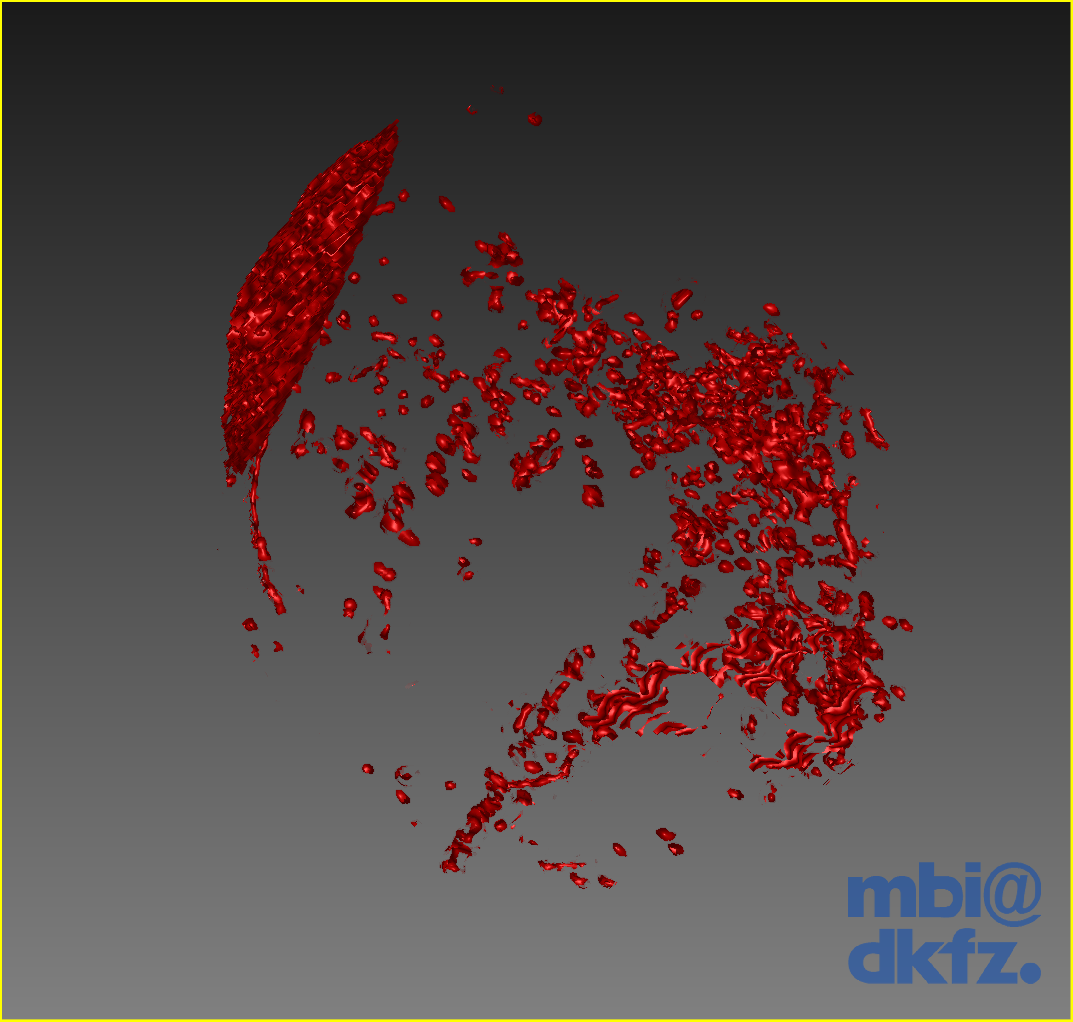
\includegraphics[width=\textwidth]{images/thresholding/thresholdvariation1threshold3.png}
    \caption{Threshold 0.01}
    \label{fig:thresholdingvariation1threshold3}  
  \end{subfigure}  
  \caption{Reducing the threshold removes the edge but removes some uncertainty.}\label{fig:thresholdingvariationfix}
\end{figure}

Although tweaking the threshold can remove edge artefact variation 2 was found not to exhibit these problems and so this implementation was used in the evaluation of the prototype.

As well as allowing the user to explicitly specify a range [min, max], it is possible to find the worst $x\%$ of uncertainty. To do this a histogram is built which splits the uncertainty into $n$ buckets. The histogram is then traversed, starting from the first (least certain) bucket, and the occurrences are accumulated until the total is greater than $uncertaintyWidth \times uncertaintyHeight \times uncertaintyDepth \times \frac{x}{100}$. When the total exceeds this value the index of the bucket, $i$, is used to compute the range: [0.0, $i \times \frac{1}{n}$]. Then the thresholding is completed as before.

\subsection*{Results}
Examples of this visualization with the test uncertainties (see section \ref{method:test_uncertainties}) are shown below for illustration. The scan used in each case is a reconstructed fetal brain.

\begin{figure}[H]
  \centering
  \begin{subfigure}[b]{0.5\textwidth}
    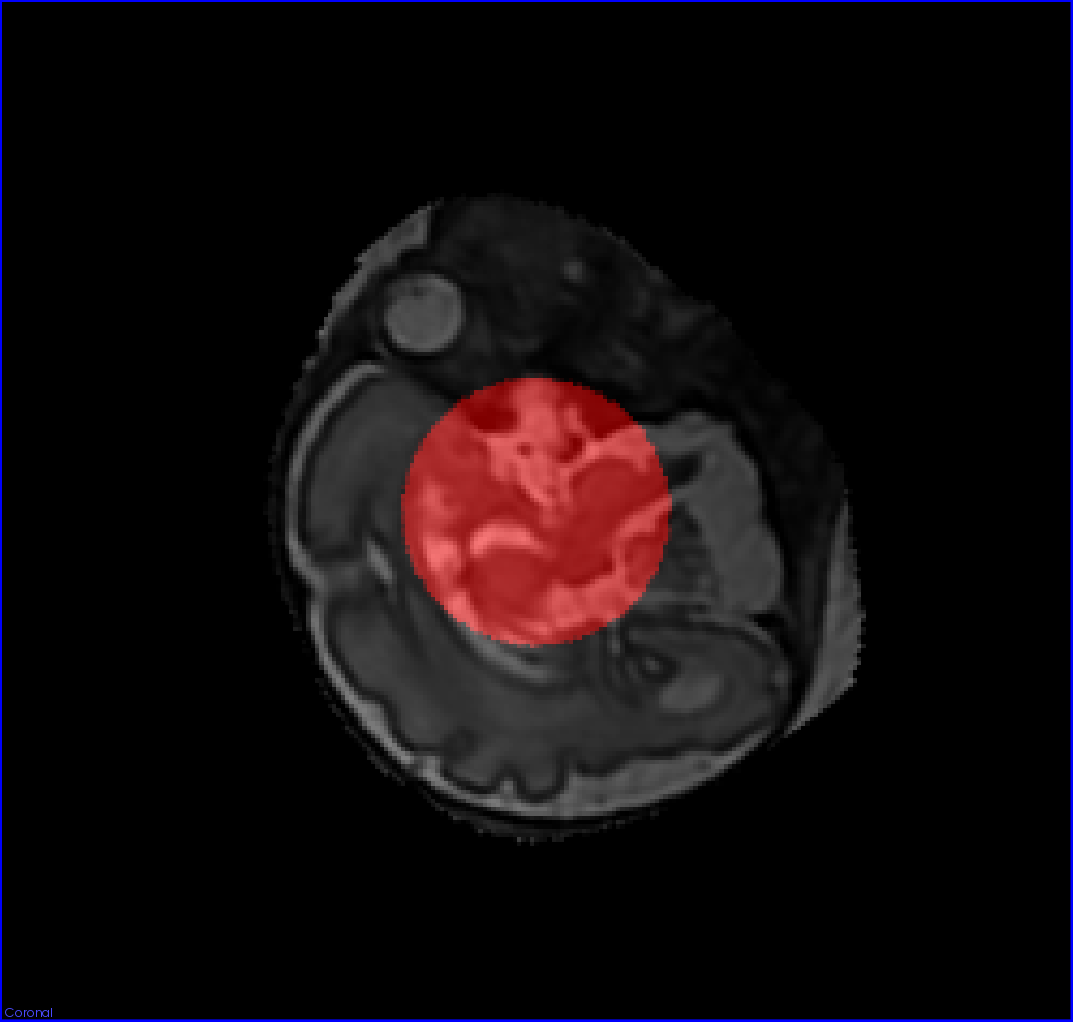
\includegraphics[width=\textwidth]{images/thresholding/results/sphere_2d.png}
    \caption{Sphere in 2D (Worst 5$\%$)}
    \label{fig:thresholdingresultssphere2d}
  \end{subfigure}%
  ~ %add desired spacing between images, e. g. ~, \quad, \qquad, \hfill etc.
    %(or a blank line to force the subfigure onto a new line)
  \begin{subfigure}[b]{0.5\textwidth}
    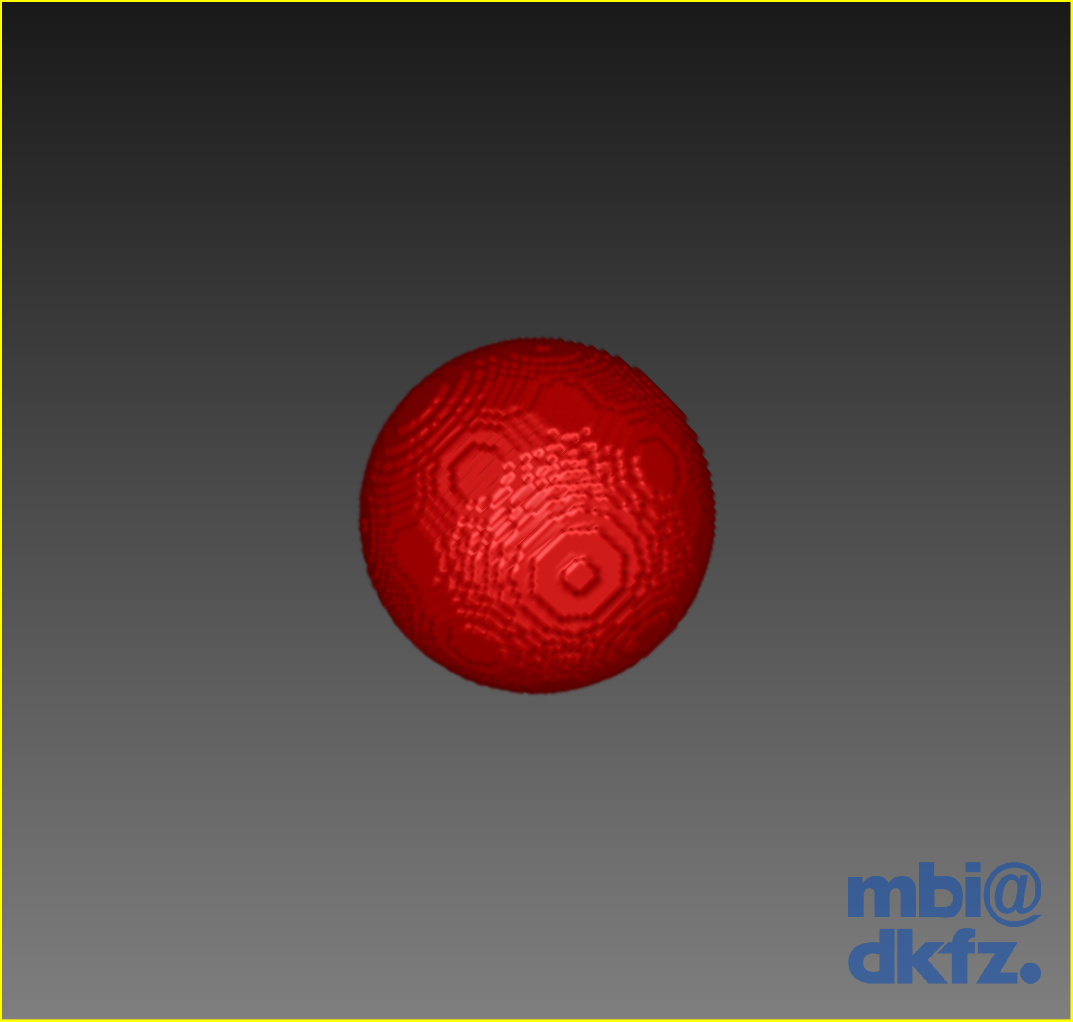
\includegraphics[width=\textwidth]{images/thresholding/results/sphere_3d.png}
    \caption{Sphere in 3D (Worst 5$\%$)}
    \label{fig:thresholdingresultssphere3d}
  \end{subfigure}\\[11pt]
  ~ %add desired spacing between images, e. g. ~, \quad, \qquad, \hfill etc.
    %(or a blank line to force the subfigure onto a new line)
  \begin{subfigure}[b]{0.5\textwidth}
    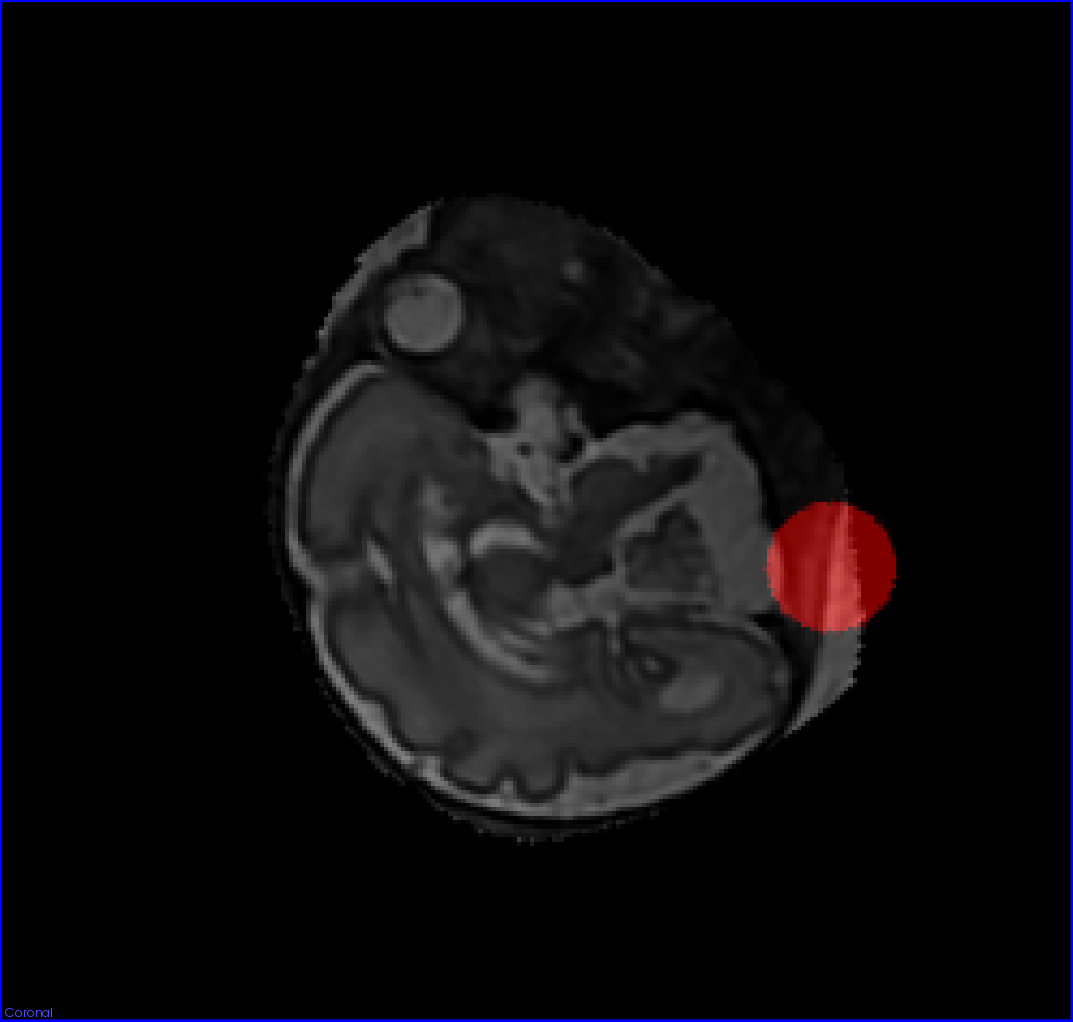
\includegraphics[width=\textwidth]{images/thresholding/results/sphere_corner_2d.png}
    \caption{Sphere in Corner in 2D (Worst 1$\%$)}
    \label{fig:thresholdingresultsspherecorner2d}
  \end{subfigure}%
  ~ %add desired spacing between images, e. g. ~, \quad, \qquad, \hfill etc.
    %(or a blank line to force the subfigure onto a new line)
  \begin{subfigure}[b]{0.5\textwidth}
    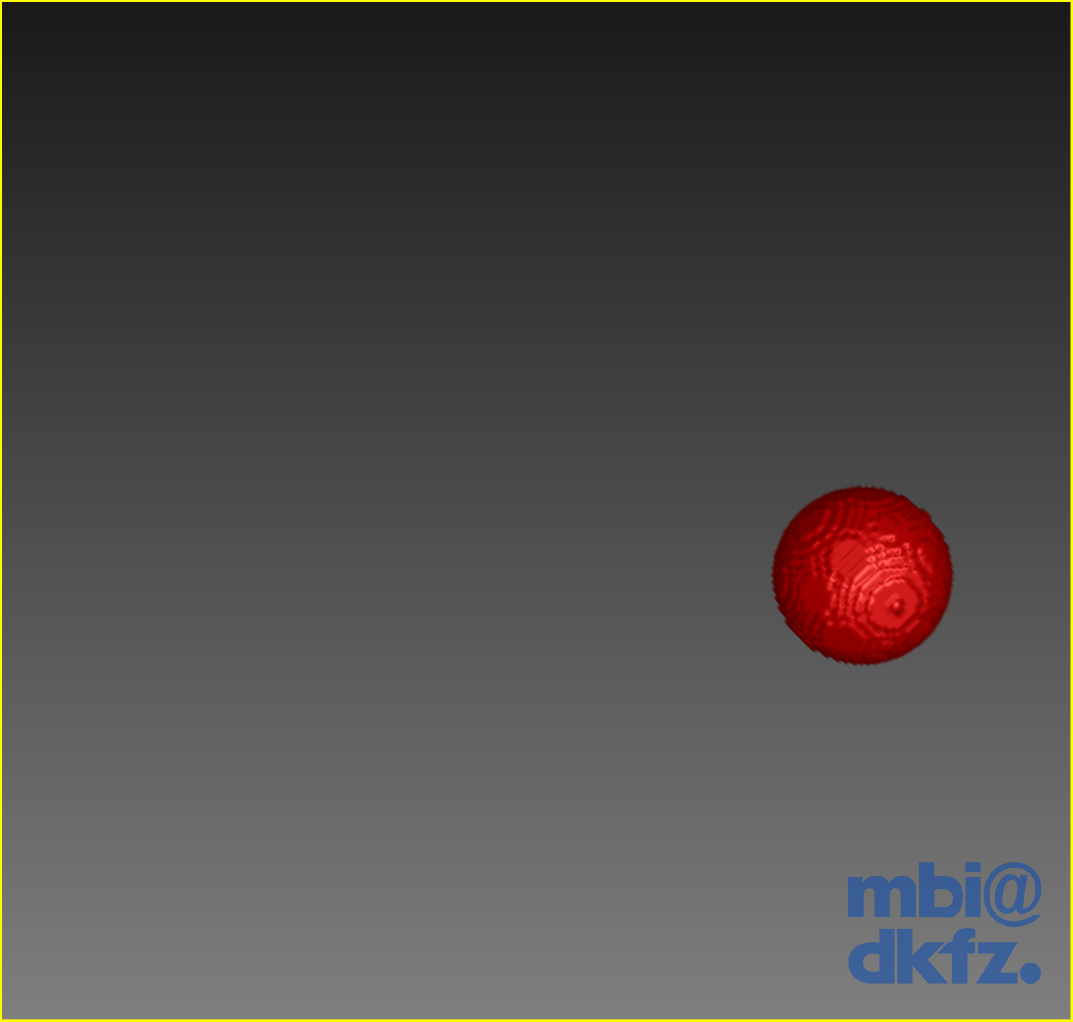
\includegraphics[width=\textwidth]{images/thresholding/results/sphere_corner_3d.png}
    \caption{Sphere in Corner in 3D (Worst 1$\%$)}
    \label{fig:thresholdingresultsspherecorner3d}
  \end{subfigure}
  % \caption{Opacity Transfer Functions. Opacity of 0 is transparent, 1 is opaque.}\label{fig:thresholdingvariation1problem}
\end{figure}

\begin{figure}[H]
  \ContinuedFloat 
  \centering
  \begin{subfigure}[b]{0.5\textwidth}
    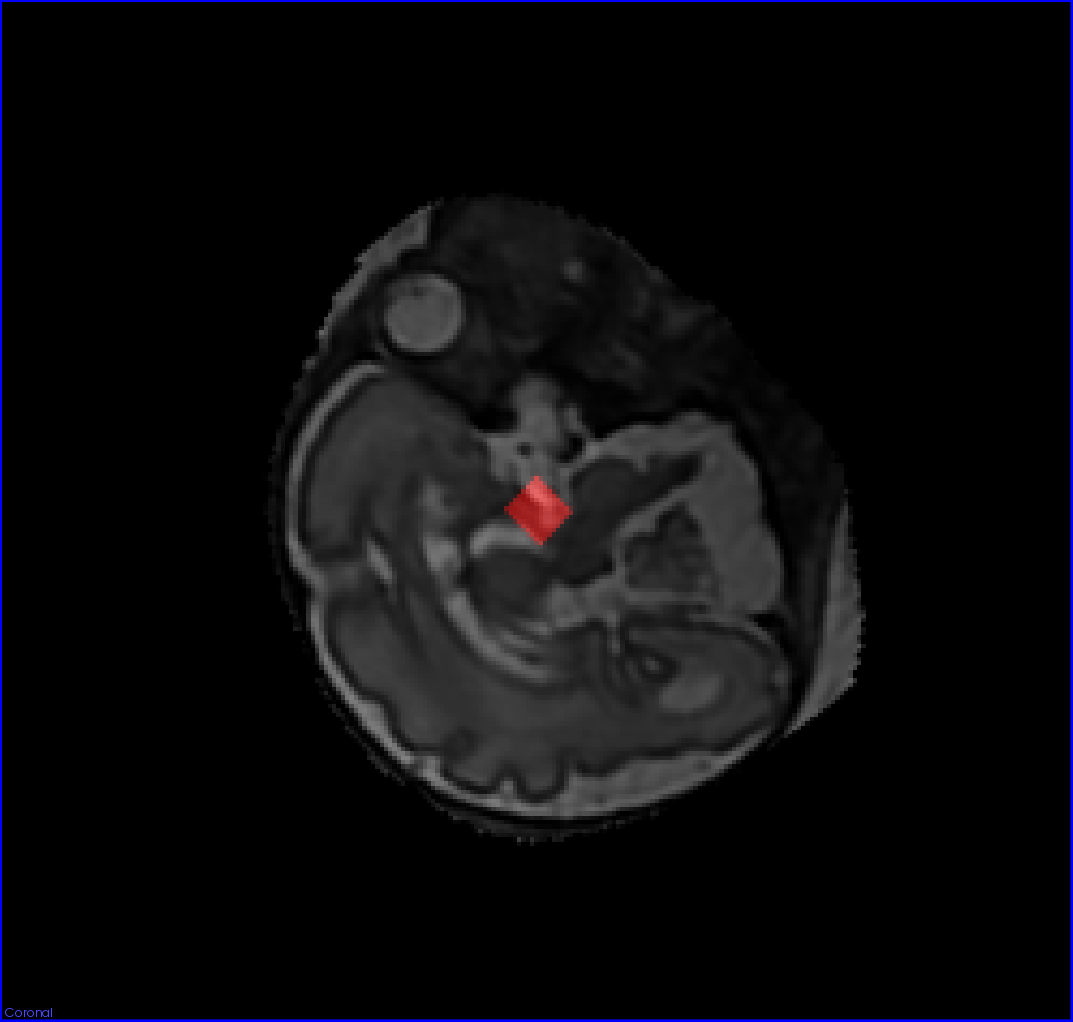
\includegraphics[width=\textwidth]{images/thresholding/results/cube_2d.png}
    \caption{Cube in 2D ([0, 0.9])}
    \label{fig:thresholdingresultscube2d}
  \end{subfigure}%
  ~ %add desired spacing between images, e. g. ~, \quad, \qquad, \hfill etc.
    %(or a blank line to force the subfigure onto a new line)
  \begin{subfigure}[b]{0.5\textwidth}
    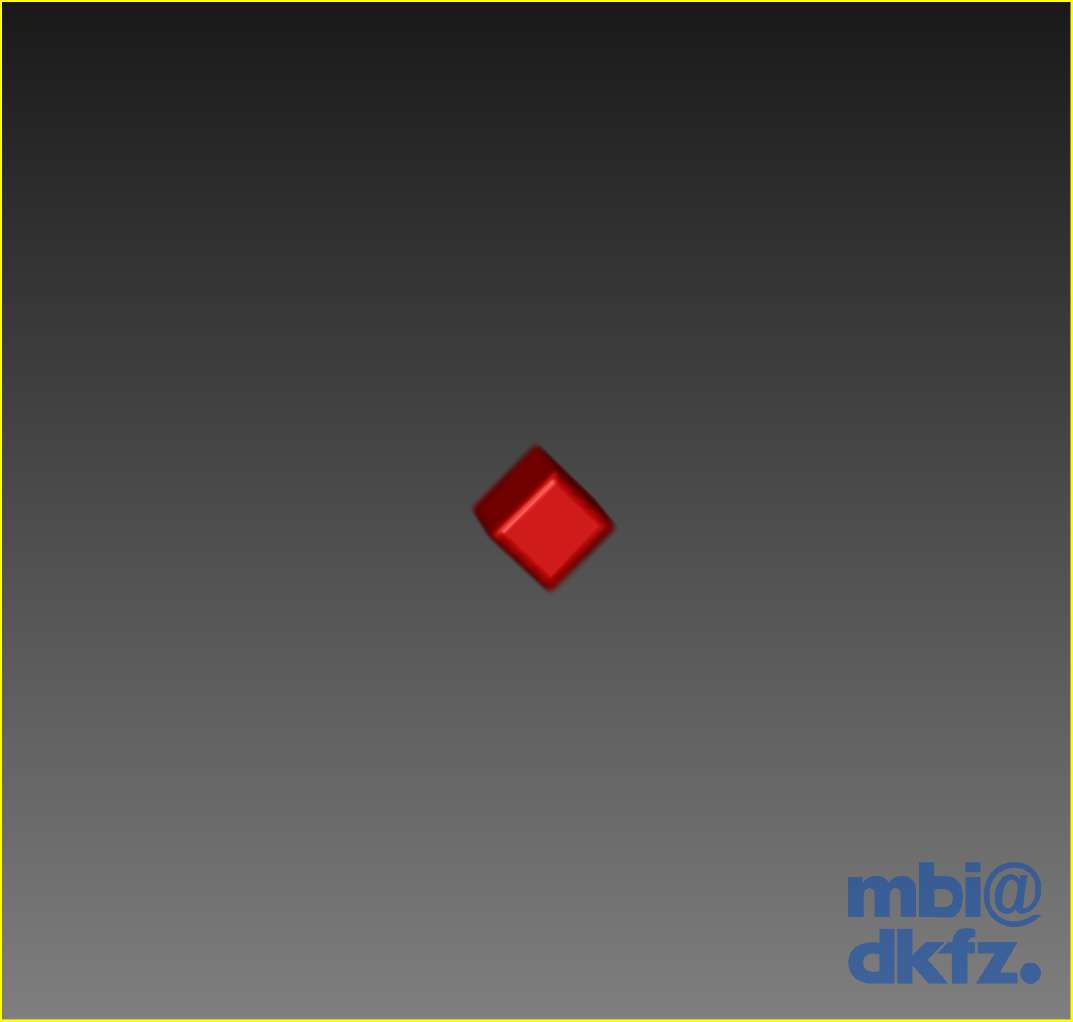
\includegraphics[width=\textwidth]{images/thresholding/results/cube_3d.png}
    \caption{Cube in 3D ([0, 0.9])}
    \label{fig:thresholdingresultscube3d}
  \end{subfigure}\\[11pt]
  ~ %add desired spacing between images, e. g. ~, \quad, \qquad, \hfill etc.
    %(or a blank line to force the subfigure onto a new line)
  \begin{subfigure}[b]{0.5\textwidth}
    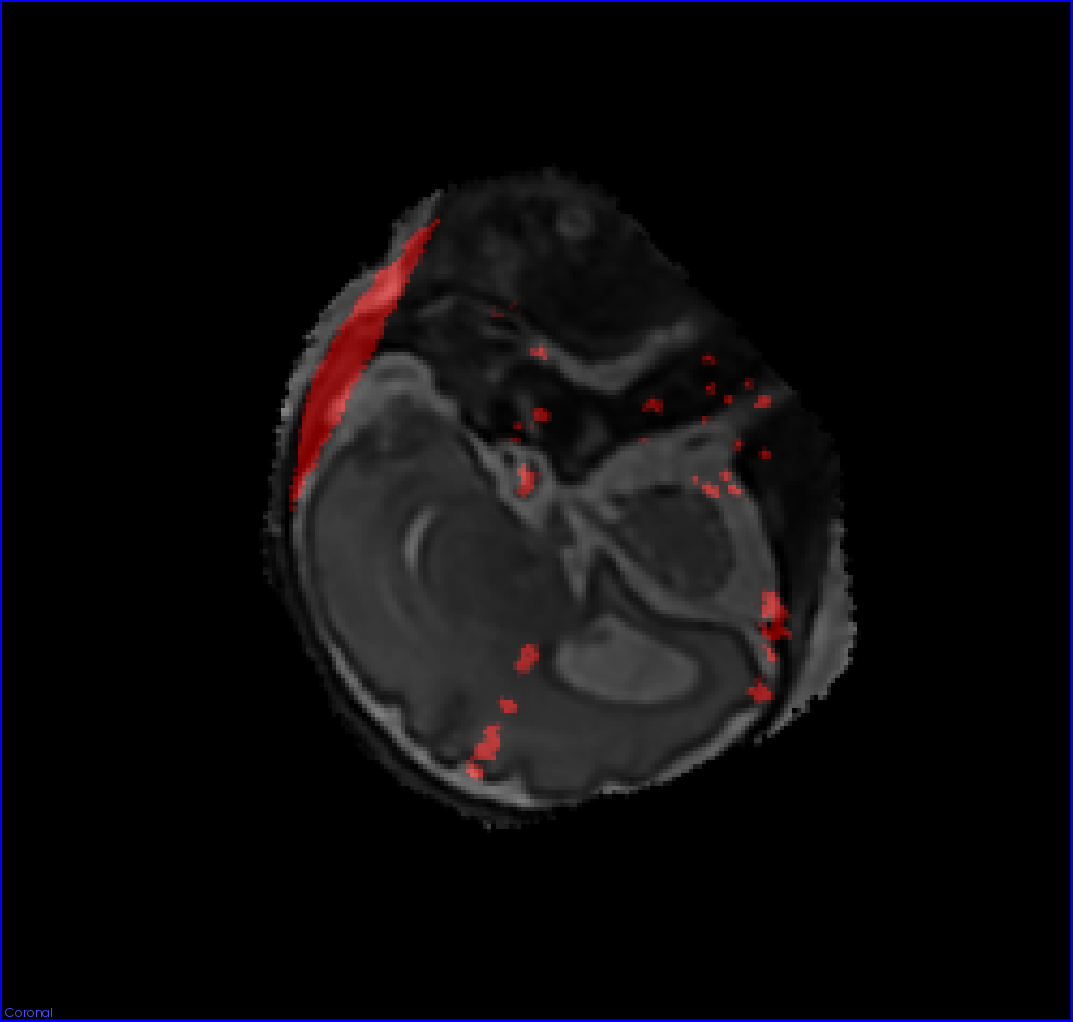
\includegraphics[width=\textwidth]{images/thresholding/results/scan_2d.png}
    \caption{Scan in 2D (Worst 5$\%$)}
    \label{fig:thresholdingresultsscan2d}
  \end{subfigure}%
  ~ %add desired spacing between images, e. g. ~, \quad, \qquad, \hfill etc.
    %(or a blank line to force the subfigure onto a new line)
  \begin{subfigure}[b]{0.5\textwidth}
    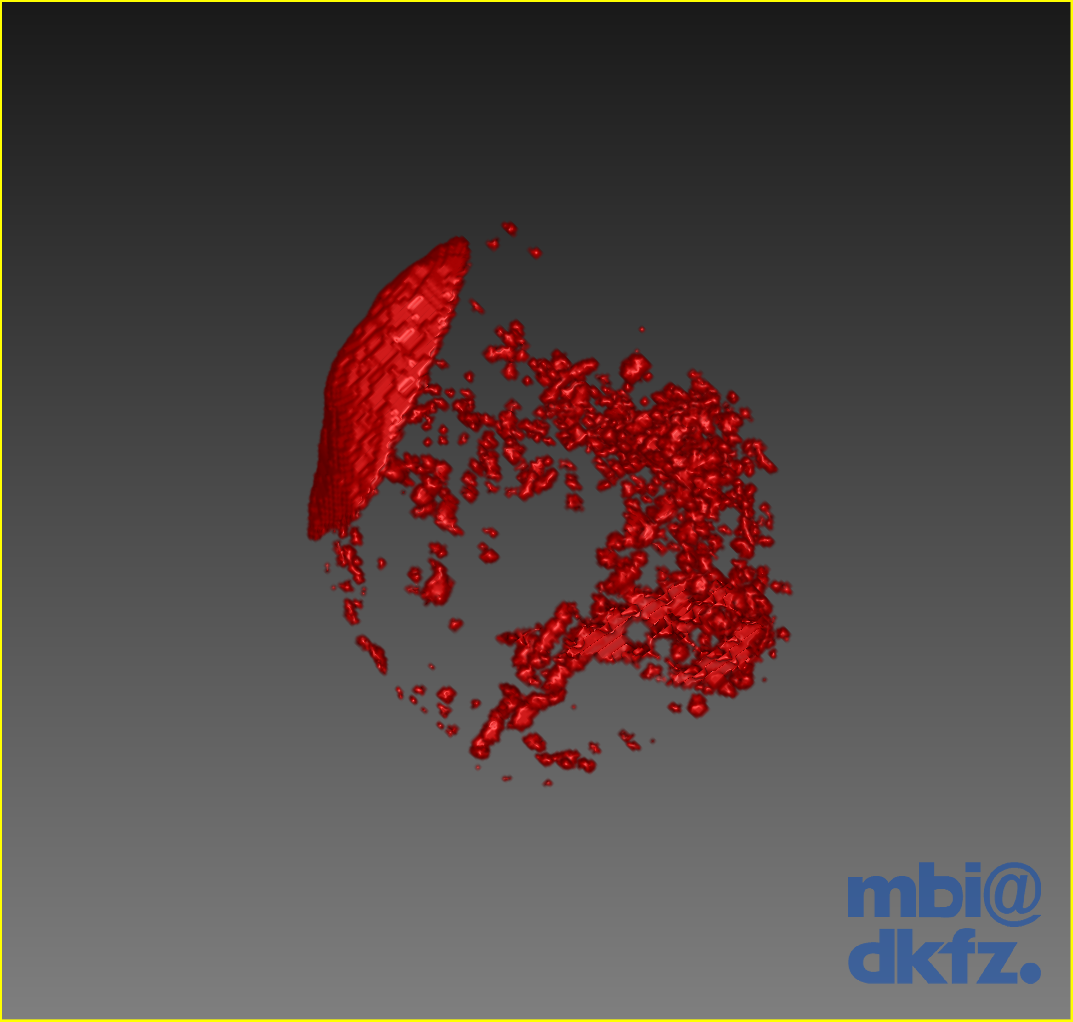
\includegraphics[width=\textwidth]{images/thresholding/results/scan_3d.png}
    \caption{Scan in 3D (Worst 5$\%$)}
    \label{fig:thresholdingresultsscan3d}
  \end{subfigure}
  % \caption{Opacity Transfer Functions. Opacity of 0 is transparent, 1 is opaque.}\label{fig:thresholdingvariation1problem}
\end{figure}

% ----------------------------- %
% ---------- SPHERE  ---------- %
% ----------------------------- %

\clearpage
\subsection{Sphere}\label{method:sphere}
The idea behind both the uncertainty sphere and uncertainty surface visualizations is to project the uncertainty, which is a 3D volume, onto a surface model, which is essentially 2D. This gives the viewer an overview of the uncertainty. Two ways of mapping the uncertainty to the surfaces have been trialled. The first builds a texture which can then be mapped to the surface.

Figure \ref{fig:uncertaintytexture} shows such a texture and the result when viewed on a sphere. The texture is generated by doing the following for each pixel:

\begin{enumerate}
  \item Convert the pixel position (x, y) to spherical coordinates ($\theta$, $\phi$). (Figure \ref{fig:texturetexture})
  \item The spherical coordinates ($\theta$, $\phi$) are then converted to the point (x', y', z') on a sphere of unit radius. (Figure \ref{fig:texturesphere})
  \item A ray is fired from the center of the uncertainty volume outwards in direction (x', y', z') and uncertainty is sampled at unit steps until the edge of the volume is reached (see volume rendering section \ref{background:volumerendering}). The average uncertainty along that ray, $u \in [0, 1]$ is then mapped to a shade of grey $((1 - u) \times 255)$.
\end{enumerate}

\savebox{\mybox}{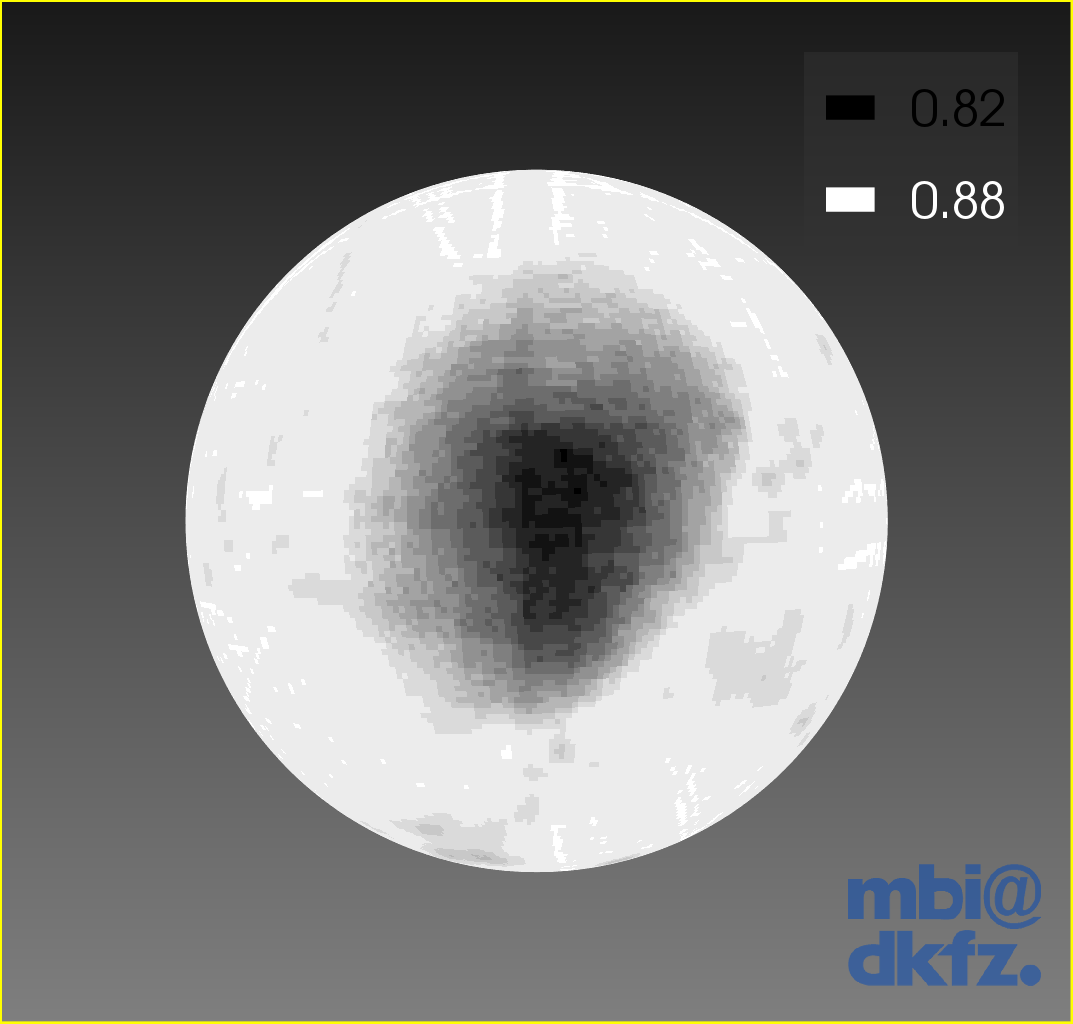
\includegraphics[width=0.5\textwidth]{images/surface/texture_sphere.png}}
\begin{figure}[H]
  \centering
  \begin{subfigure}[b]{0.5\textwidth}
    \vbox to \ht\mybox{%
      \vfill
      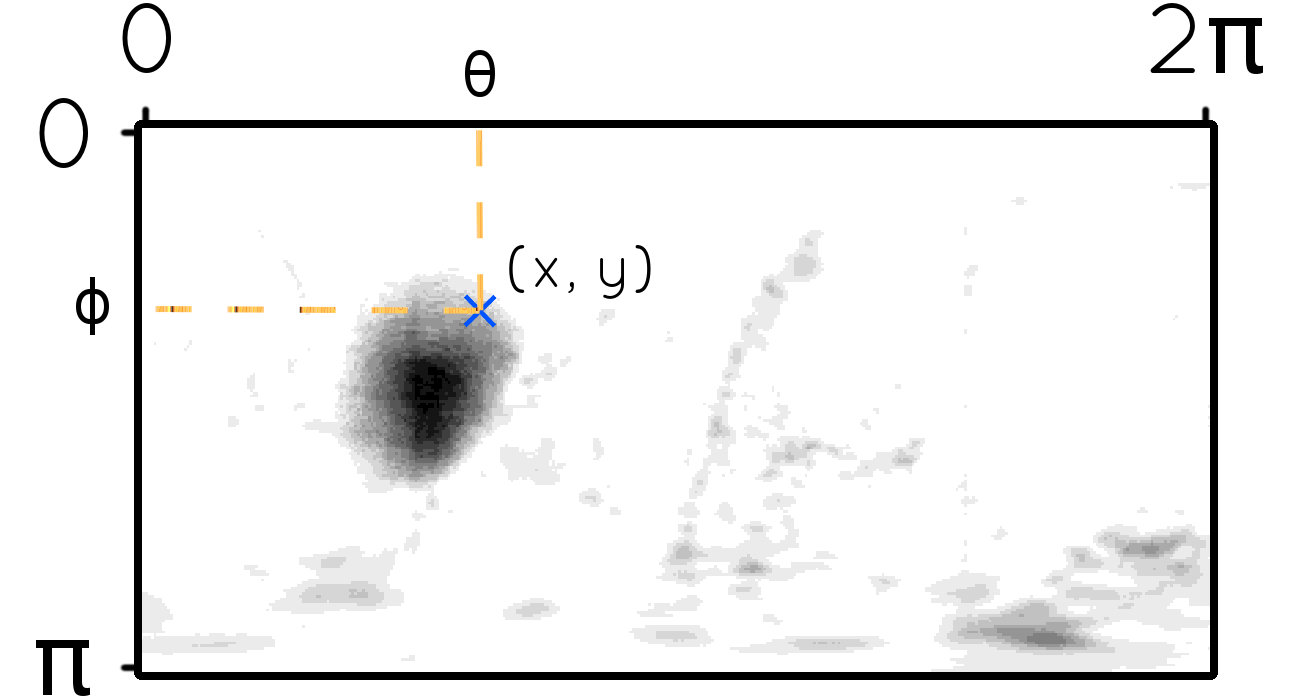
\includegraphics[width=\textwidth]{images/surface/spherical_1.png}
      \vfill
    }
    \caption{Uncertainty Texture}
    \label{fig:texturetexture}
  \end{subfigure}%
  ~ %add desired spacing between images, e. g. ~, \quad, \qquad, \hfill etc.
    %(or a blank line to force the subfigure onto a new line)
  \begin{subfigure}[b]{0.5\textwidth}
    \usebox{\mybox}
    \caption{Mapped to Sphere}
    \label{fig:texturesphere}
  \end{subfigure}
  \caption{Mapping a texture to a sphere.}\label{fig:uncertaintytexture}
\end{figure}

This technique has a number of issues. Firstly, it looks quite blocky unless the resolution is set very high. Secondly, due to the conversion to spherical coordinates parts of the sphere are less well represented; in particular all pixels in the top row correspond to the very top of the sphere. Finally this technique does not translate very well when trying to map to arbitrary surfaces that are not as regular as a sphere.

Another approach was then trialled. Instead of mapping the uncertainty to a texture a colour is directly stored at each point in the surface representation and these values are used to interpolate values all over the surface.

This process begins by generating a surface representation of a sphere. In the same way that the resolution of the texture could be increased, more points can be used to model the sphere. Modelling in this way removes the issue that the top of the sphere is over-represented; there is only ever one point at the top.

Then each point on the sphere is registered to a start point in the volume (Fig. \ref{fig:surface_sampling_example}: Volume Intersection). This is done by testing the intersection of the ray (a line) with the six faces (planes) of the volume to decide which is hit first.

Sampling then begins in the direction of the normal until the start of the object (and not the background) is found (Fig. \ref{fig:surface_sampling_example}: Uncertainty Intersection).

\begin{figure}[H]
  \centering
  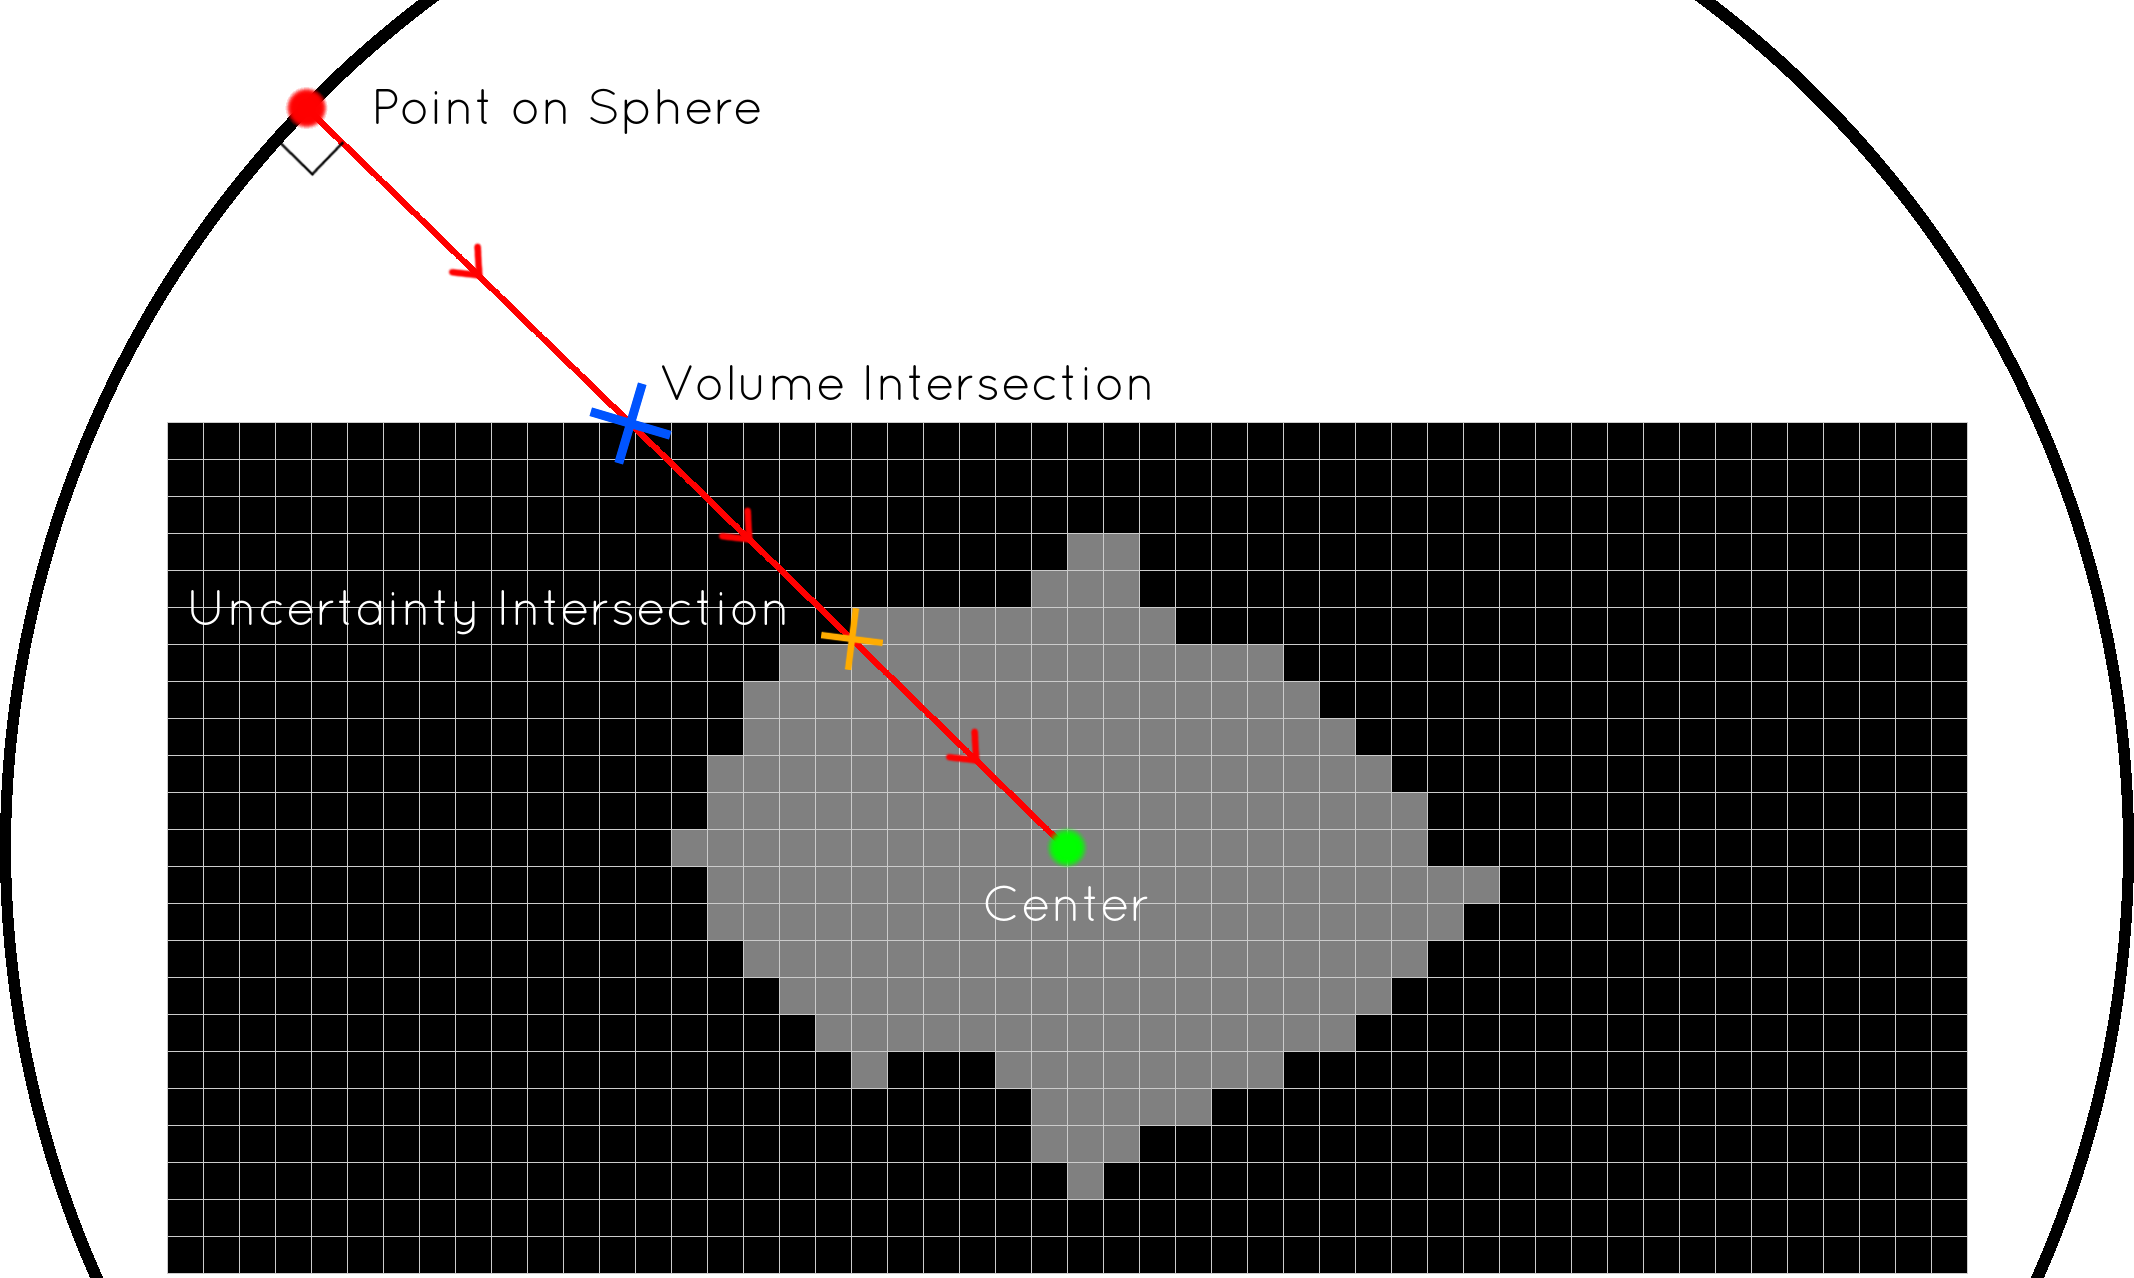
\includegraphics[width=\textwidth]{images/surface/sampling_example.png}
  \caption{Sampling Overview}\label{fig:surface_sampling_example}
\end{figure}

A tortoise and hare algorithm is then used to be able to vary how far into the volume the sampling goes. The tortoise moves through the uncertainty accumulating samples whilst the hare shoots off trying to find the edge. When the hare does find the edge the sampling stops. If the hare travels at the same speed as the tortoise then the entire object is sampled, if it travels at twice the speed of the tortoise then the sampling stops half the way through and so on. This is illustrated in figure \ref{fig:tortoiseandhareexample}.

\begin{figure}[H]
  \centering
  \begin{subfigure}[b]{0.32\textwidth}
    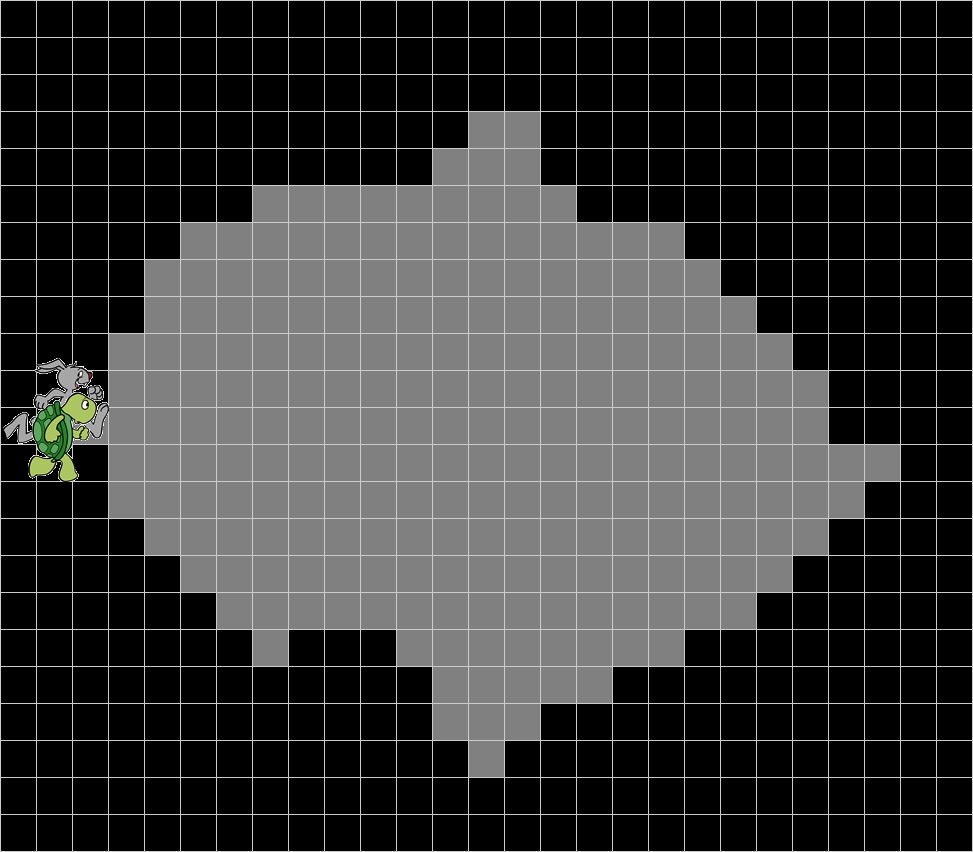
\includegraphics[width=\textwidth]{images/surface/tortoise_and_hare_1.png}
    \caption*{Start}
    \label{fig:tortoiseandhare1}
  \end{subfigure}%
  ~ %add desired spacing between images, e. g. ~, \quad, \qquad, \hfill etc.
    %(or a blank line to force the subfigure onto a new line)
  \begin{subfigure}[b]{0.32\textwidth}
    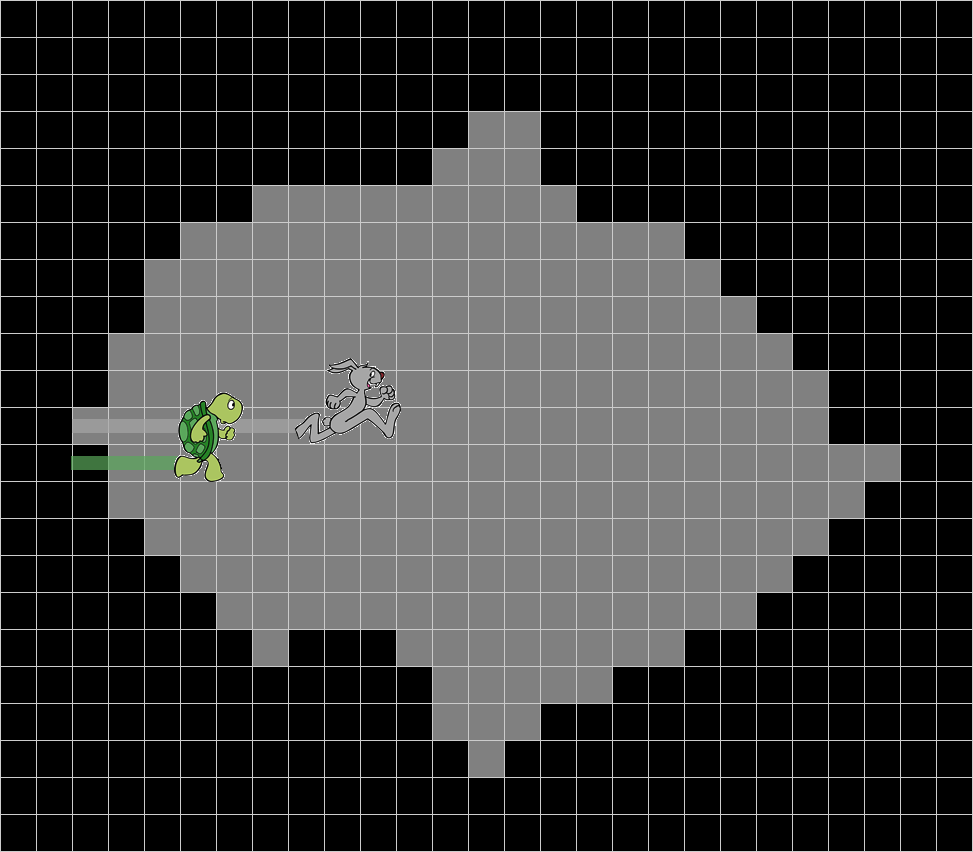
\includegraphics[width=\textwidth]{images/surface/tortoise_and_hare_2.png}
    \caption*{...}
    \label{fig:tortoiseandhare2}
  \end{subfigure}%
  ~ %add desired spacing between images, e. g. ~, \quad, \qquad, \hfill etc.
    %(or a blank line to force the subfigure onto a new line)
  \begin{subfigure}[b]{0.32\textwidth}
    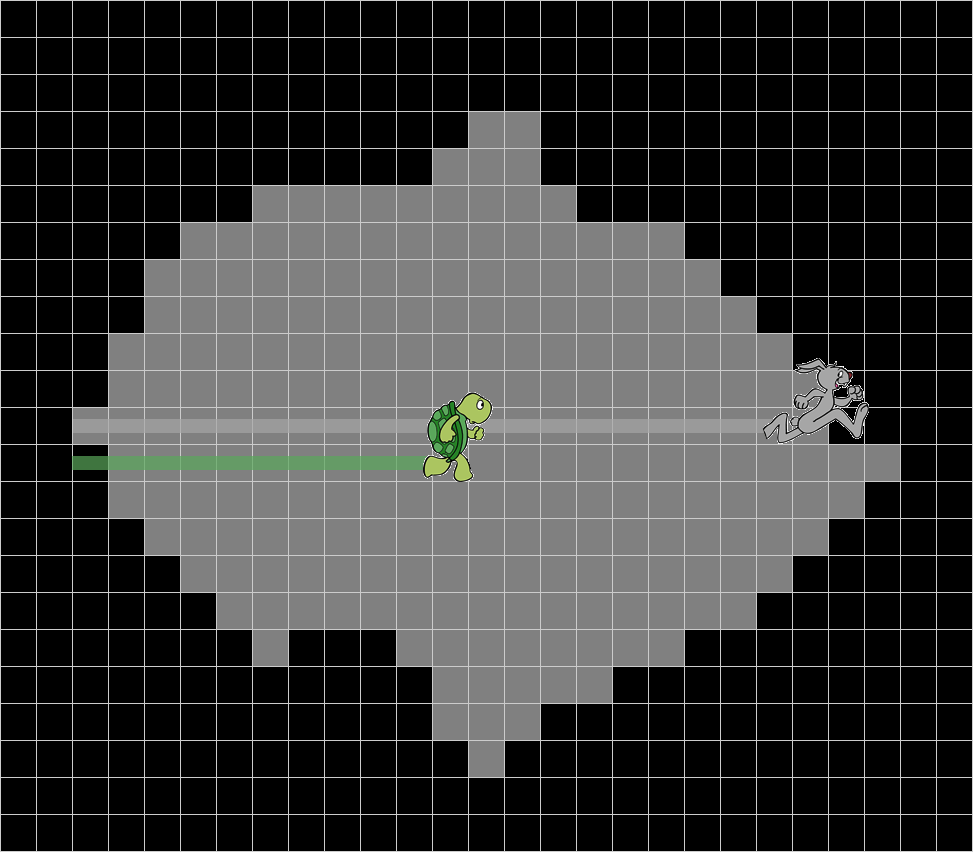
\includegraphics[width=\textwidth]{images/surface/tortoise_and_hare_3.png}
    \caption*{End}
    \label{fig:tortoiseandhare3}  
  \end{subfigure}
  \caption{Illustration of Tortoise and Hare Algorithm}\label{fig:tortoiseandhareexample}
\end{figure}

The accumulation that the tortoise does can also be customized. The average of all the samples can be taken, but also the best and worst values along the ray can be extracted.

Once all of the points have been computed some scaling can be implemented to improve the contrast of the visualization. In many cases the average uncertainty will be roughly the same everywhere and if the range [0-1] is mapped to the entire colour range the values end up looking largely indistinguishable; to fix this the outputted uncertainty range can be linearly mapped to make better use of the available colours.

% ----------------------------- %
% ---------- SURFACE ---------- %
% ----------------------------- %

\subsection{Surface}\label{method:surface}
In addition to mapping the uncertainty to a generic representation, the sphere, it is also possible to map it to a surface representation of the object being scanned. The procedure is largely the same as before. Firstly the surface is generated by taking the mask used in the reconstruction and applying surface extraction (see section \ref{background:surfaceextraction}). The raw surface created in this way is shown in figure \ref{fig:surfaceraw}.

\begin{wrapfigure}[5]{r}{0.4\textwidth}
  \vspace{-20pt}
  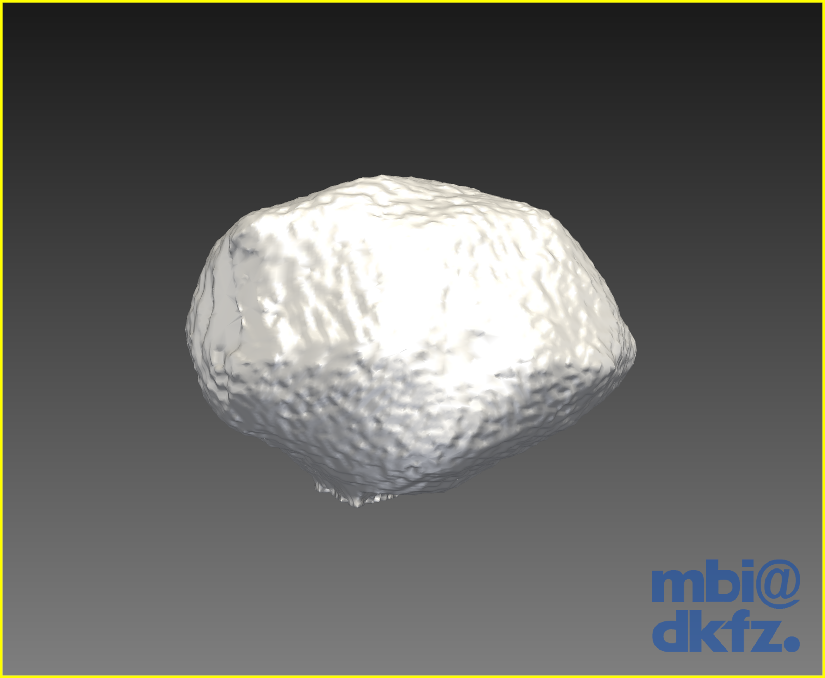
\includegraphics[width=0.4\textwidth]{images/surface/surface_raw.png}
  \caption{Extracted Surface}\label{fig:surfaceraw}
\end{wrapfigure}

The registration step is then trivial as the mask, and therefore the surface, use the same coordinate system as the uncertainty volume. Then the sampling continues exactly as before with the normal at the surface used as the direction to sample in.

\newpage
\subsection*{Results}
Scaling was found to significantly increase the contrast of the visualization, see figure \ref{fig:surfacescaling}. The legend overlayed shows the scaling applied in each case.

\begin{figure}[H]
  \centering
  \begin{subfigure}[b]{0.5\textwidth}
    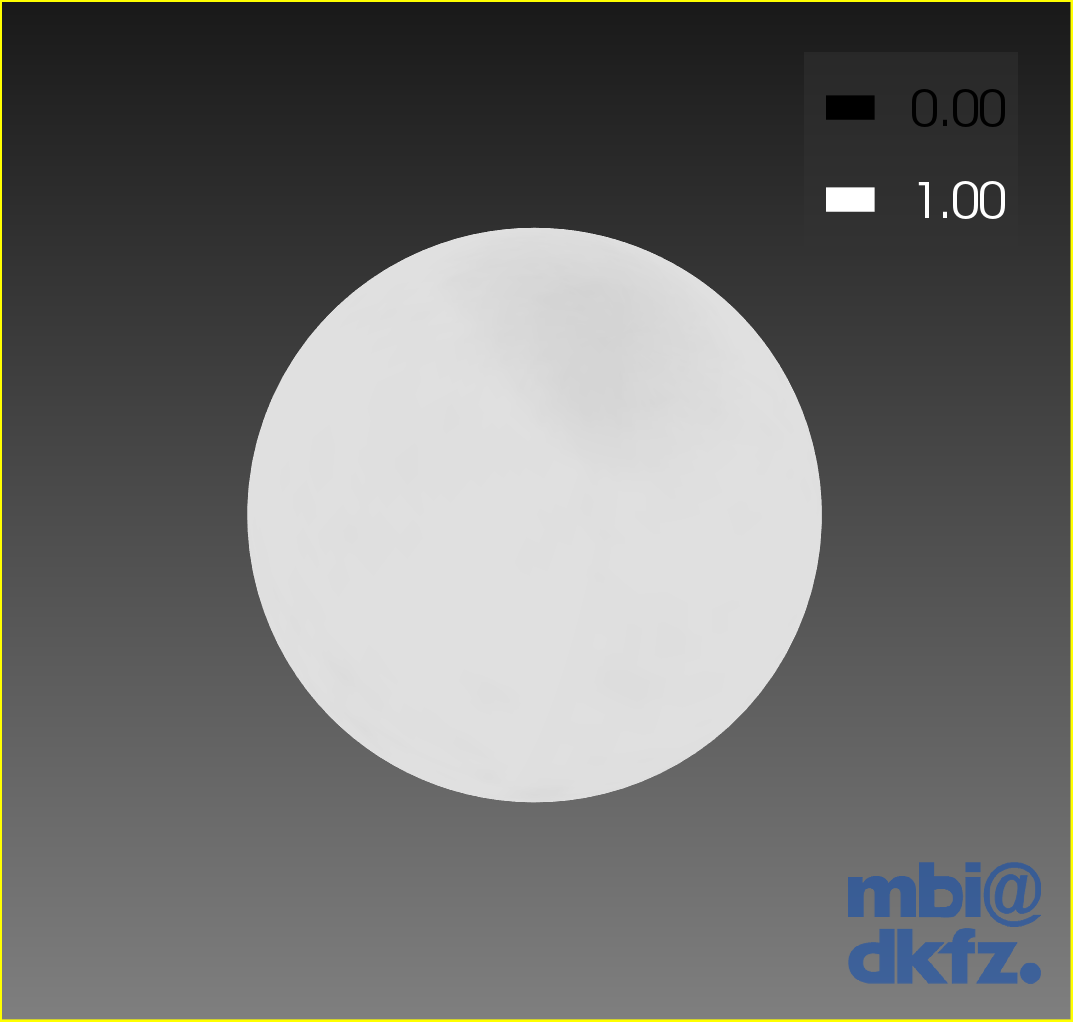
\includegraphics[width=\textwidth]{images/surface/sphere_no_scaling.png}
    \caption*{Sphere\\(No Scaling)}
    \label{fig:surfacespherenoscaling}
  \end{subfigure}%
    %add desired spacing between images, e. g. ~, \quad, \qquad, \hfill etc.
    %(or a blank line to force the subfigure onto a new line)
  \begin{subfigure}[b]{0.5\textwidth}
    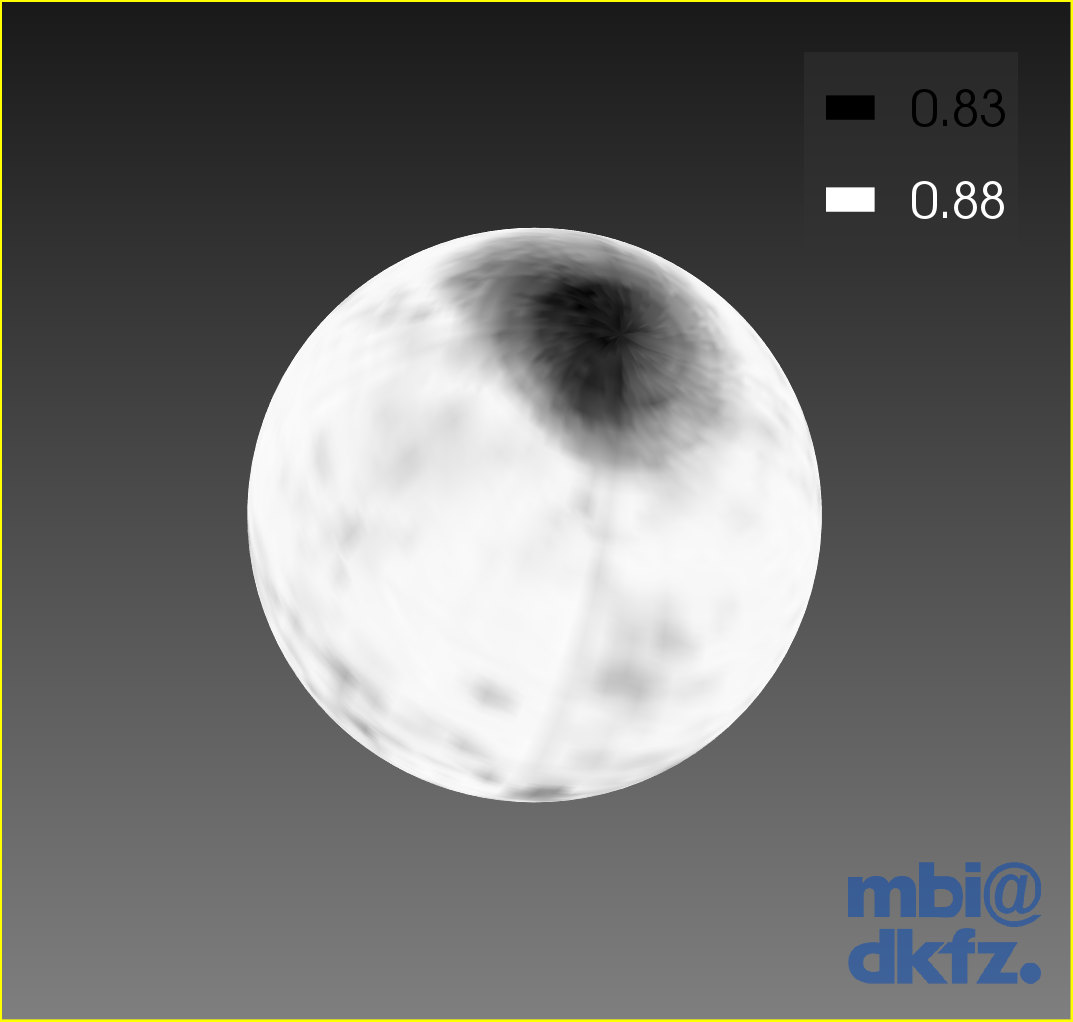
\includegraphics[width=\textwidth]{images/surface/sphere_scaling.png}
    \caption*{Sphere\\(Linear)}
    \label{fig:surfacespherescaling}
  \end{subfigure}\\[11pt]
    %add desired spacing between images, e. g. ~, \quad, \qquad, \hfill etc.
    %(or a blank line to force the subfigure onto a new line)
  \begin{subfigure}[b]{0.5\textwidth}
    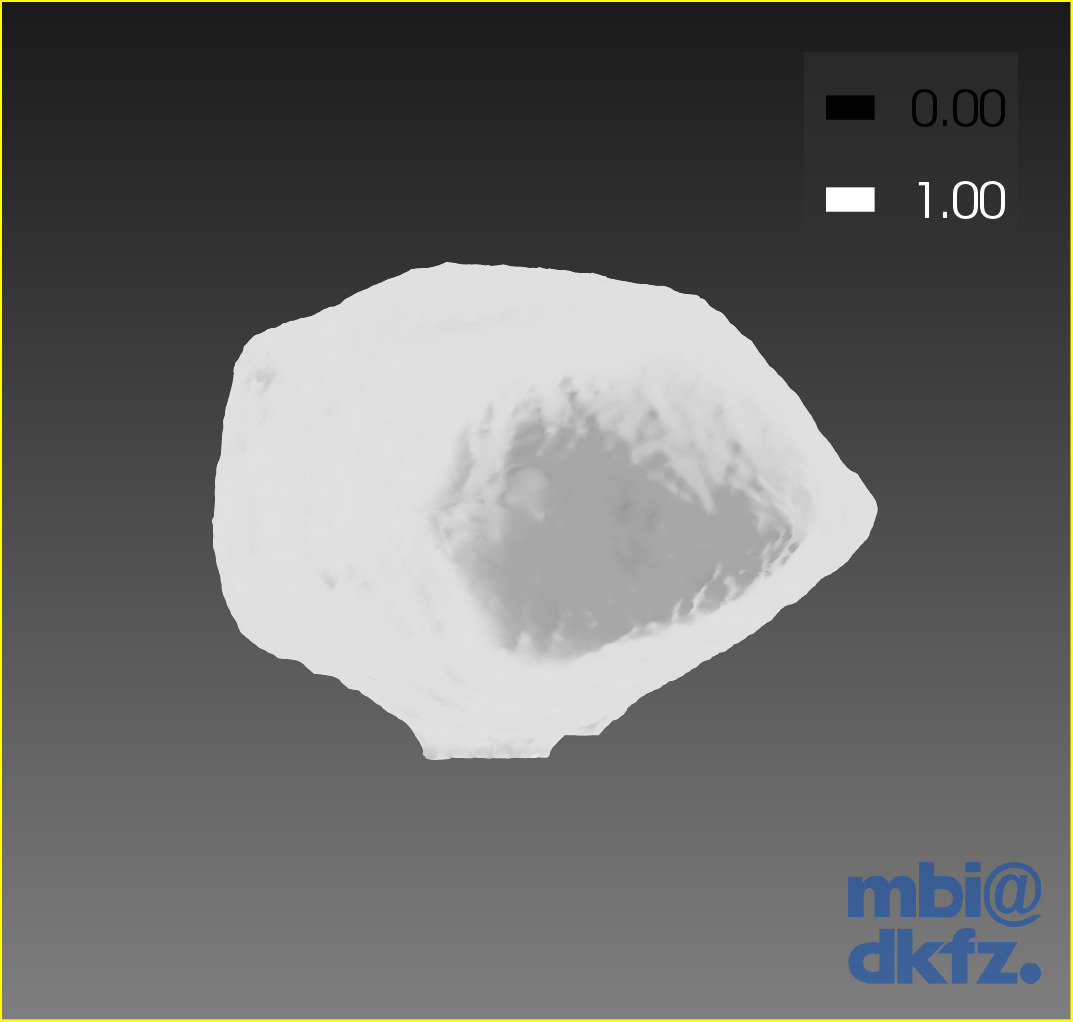
\includegraphics[width=\textwidth]{images/surface/surface_no_scaling.png}
    \caption*{Surface\\(No Scaling)}
    \label{fig:surfacesurfacenoscaling}
  \end{subfigure}%
    %add desired spacing between images, e. g. ~, \quad, \qquad, \hfill etc.
    %(or a blank line to force the subfigure onto a new line)
  \begin{subfigure}[b]{0.5\textwidth}
    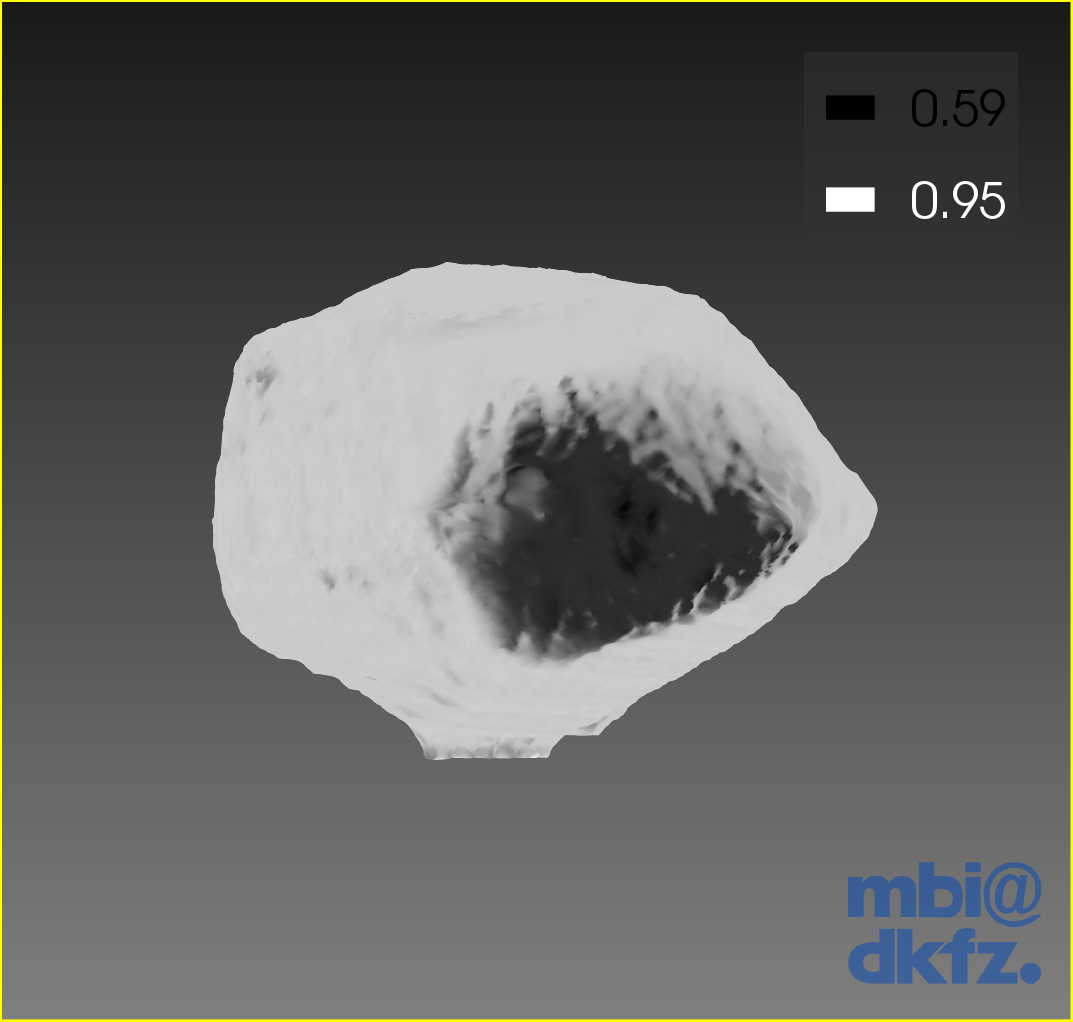
\includegraphics[width=\textwidth]{images/surface/surface_scaling.png}
    \caption*{Sphere\\(Linear)}
    \label{fig:surfacesurfacescaling}
  \end{subfigure}
  \caption{The effect of linear mapping.}\label{fig:surfacescaling}
\end{figure}

The surface representation difficult to interpret by looking at a single image on paper. Figure \ref{fig:surface180} shows the surface from various angles. In practice all of these visualizations can be rotated and zoomed.

\begin{figure}[h]
  \centering
  \begin{subfigure}[b]{0.20\textwidth}
    \includegraphics[width=\textwidth]{images/surface/surface_180_1.png}
    \caption*{Left}
    \label{fig:surface_left}
  \end{subfigure}%
    %add desired spacing between images, e. g. ~, \quad, \qquad, \hfill etc.
    %(or a blank line to force the subfigure onto a new line)
  \begin{subfigure}[b]{0.20\textwidth}
    \includegraphics[width=\textwidth]{images/surface/surface_180_2.png}
    \caption*{Front Left}
    \label{fig:surface_front_left}
  \end{subfigure}%
    %add desired spacing between images, e. g. ~, \quad, \qquad, \hfill etc.
    %(or a blank line to force the subfigure onto a new line)
  \begin{subfigure}[b]{0.20\textwidth}
    \includegraphics[width=\textwidth]{images/surface/surface_180_3.png}
    \caption*{Front}
    \label{fig:surface_front}
  \end{subfigure}%
    %add desired spacing between images, e. g. ~, \quad, \qquad, \hfill etc.
    %(or a blank line to force the subfigure onto a new line)
  \begin{subfigure}[b]{0.20\textwidth}
    \includegraphics[width=\textwidth]{images/surface/surface_180_4.png}
    \caption*{Front Right}
    \label{fig:surface_front_right}
  \end{subfigure}%
    %add desired spacing between images, e. g. ~, \quad, \qquad, \hfill etc.
    %(or a blank line to force the subfigure onto a new line)
  \begin{subfigure}[b]{0.20\textwidth}
    \includegraphics[width=\textwidth]{images/surface/surface_180_5.png}
    \caption*{Right}
    \label{fig:surface_right}
  \end{subfigure}
  \caption{Brain surface viewed from different directions.}\label{fig:surface180}
\end{figure}

Figure \ref{fig:surfaceaccumulator} illustrates the effect of changing the accumulator. The default behaviour of taking the average uncertainty along the ray does a reasonable job of bringing the uncertainty to the surface. Changing it to extract the worst value gives the viewer a better idea of the size of the uncertain region as values that would otherwise be outweighed by largely good values are brought to the surface.

There results when finding the best value are poor. It doesn't really work at all when applied to the sphere as in the vast majority of cases there is a good value somewhere along the ray which results in a largely uniform appearance. 

The same logic largely applies to the brain surface as well, however areas on the volume where the normal does not send the ray far into the volume are visible.

\begin{figure}[H]
  \centering
  \begin{subfigure}[b]{0.32\textwidth}
    \includegraphics[width=\textwidth]{images/surface/sphere_average.png}
    \caption*{Sphere - Average}
    \label{fig:sphereaverage}
  \end{subfigure}%
  ~ %add desired spacing between images, e. g. ~, \quad, \qquad, \hfill etc.
    %(or a blank line to force the subfigure onto a new line)
  \begin{subfigure}[b]{0.32\textwidth}
    \includegraphics[width=\textwidth]{images/surface/sphere_worst.png}
    \caption*{Sphere - Worst}
    \label{fig:sphereworst}
  \end{subfigure}%
  ~ %add desired spacing between images, e. g. ~, \quad, \qquad, \hfill etc.
    %(or a blank line to force the subfigure onto a new line)
  \begin{subfigure}[b]{0.32\textwidth}
    \includegraphics[width=\textwidth]{images/surface/sphere_best.png}
    \caption*{Sphere - Best}
    \label{fig:spherebest}  
  \end{subfigure}
  ~ %add desired spacing between images, e. g. ~, \quad, \qquad, \hfill etc.
    %(or a blank line to force the subfigure onto a new line)  
  \begin{subfigure}[b]{0.32\textwidth}
    \includegraphics[width=\textwidth]{images/surface/surface_average.png}
    \caption*{Surface - Average}
    \label{fig:surfaceaverage}
  \end{subfigure}%
  ~ %add desired spacing between images, e. g. ~, \quad, \qquad, \hfill etc.
    %(or a blank line to force the subfigure onto a new line)
  \begin{subfigure}[b]{0.32\textwidth}
    \includegraphics[width=\textwidth]{images/surface/surface_worst.png}
    \caption*{Surface - Worst}
    \label{fig:surfaceworst}
  \end{subfigure}%
  ~ %add desired spacing between images, e. g. ~, \quad, \qquad, \hfill etc.
    %(or a blank line to force the subfigure onto a new line)
  \begin{subfigure}[b]{0.32\textwidth}
    \includegraphics[width=\textwidth]{images/surface/surface_best.png}
    \caption*{Surface - Best}
    \label{fig:surfacebest}  
  \end{subfigure}  
  \caption{Comparison of Average/Best/Worst sampling.}\label{fig:surfaceaccumulator}
\end{figure}

The sample distance determines how far into the volume samples go. Currently there are two options available - half and full. These options are less applicable to the sphere as if it is set to full then opposite sides of the sphere give identical values.

When applied to the surface the use of this option very much depends on the area of the body that is being scanned. The brain is a large, and for the most part (ignoring folds particularly) convex; in this respect it is similar to the sphere and the effect of sampling all the way through is much the same (see figure \ref{fig:surfacesampledistance}). Note that the average uncertainty gets better with full sampling as there are more good points to outweigh the bad ones in that region.\\\\

\begin{figure}[H]
  \centering
  \begin{subfigure}[b]{0.5\textwidth}
    \includegraphics[width=\textwidth]{images/surface/surface_half.png}
    \caption{Half}
    \label{fig:surfacehalf}
  \end{subfigure}%
  ~ %add desired spacing between images, e. g. ~, \quad, \qquad, \hfill etc.
    %(or a blank line to force the subfigure onto a new line)
  \begin{subfigure}[b]{0.5\textwidth}
    \includegraphics[width=\textwidth]{images/surface/surface_full.png}
    \caption{Full}
    \label{fig:surfacefull}
  \end{subfigure}
  \caption{Comparing half and full distance sampling.}\label{fig:surfacesampledistance}
\end{figure}

Where this parameter may be more useful however is when dealing with smaller, more intricate objects, such as arteries. It would allow the uncertainty in the entire cross section to be mapped to the surface, giving an overview of that section at a glance, rather than having to rotate around it to get the full picture.

% ----------------------------- %
% ------ NEXT SCAN PLANE ------ %
% ----------------------------- %

\clearpage
\subsection{Next Scan Plane}\label{method:next_scan_plane}
The idea behind this visualization is based on research\cite{uncertaintysvd} which uses SVD to find the optimum position and direction to scan next given the current uncertainty. With this knowledge the scanning process can continually target areas of uncertainty to optimize the quality of the reconstruction.

The first step in this technique is to build a list of points to target. This is done by finding all points in the uncertainty volume that are worse than a user specified threshold, in a very similar manner to the thresholding visualization. The center, $c$, of these points is then computed by taking the mean; $c$ is the position of the center of the scan.

Then a matrix of de-meaned points is created, $M = [p_1; p_2; ... ; p_n]$. SVD is then applied to $M$ (see SVD section \ref{background:svdpca}) and the direction, $d$, can be extracted. 

The center point, $c$, and direction, $d$, are then used to create a circle which represents the central slice in the scan and a cylinder to show the direction of the scan.

\subsection*{Results}
Figure \ref{fig:nextscanplanespheres} shows the next scan planes for both the sphere uncertainties. Since they both have infinitely many lines of symmetry they can be scanned from any direction.

\begin{figure}[H]
  \centering
  \begin{subfigure}[b]{0.4\textwidth}
    \includegraphics[width=\textwidth]{images/next_scan_plane/sphere.png}
    \caption{Sphere}
    \label{fig:nextscanplanesphere}
  \end{subfigure}%
  ~ %add desired spacing between images, e. g. ~, \quad, \qquad, \hfill etc.
    %(or a blank line to force the subfigure onto a new line)
  \begin{subfigure}[b]{0.4\textwidth}
    \includegraphics[width=\textwidth]{images/next_scan_plane/sphere_in_corner.png}
    \caption{Sphere in Corner}
    \label{fig:nextscanplanespherecorner}
  \end{subfigure}
  \caption{Next scan planes for the spheres.}\label{fig:nextscanplanespheres}
\end{figure}

\newpage
Figure \ref{fig:nextscanplanecube} shows the cube of uncertainty. The optimal scan is slightly counter intuitive but the scan does in fact split the uncertainty in half. See figure \ref{fig:nextscanplanecubecut}.\\\\

\savebox{\mybox}{\includegraphics[width=0.5\textwidth]{images/next_scan_plane/cube.png}}
\begin{figure}[H]
  \centering
  \begin{subfigure}[b]{0.5\textwidth}
    \usebox{\mybox}
    \caption{Cube}
    \label{fig:nextscanplanecubecube}  
  \end{subfigure}%
  ~ %add desired spacing between images, e. g. ~, \quad, \qquad, \hfill etc.
    %(or a blank line to force the subfigure onto a new line)
  \begin{subfigure}[b]{0.5\textwidth}
    \vbox to \ht\mybox{%
      \vfill
      \includegraphics[width=\textwidth]{images/next_scan_plane/cubecut.png}
      \vfill
    }
    \caption{Two halves. Image from \cite{cuttingupcubes}}
    \label{fig:nextscanplanecubecut}  
  \end{subfigure}  
  \caption{Next scan plane for the cube.}\label{fig:nextscanplanecube}
\end{figure}

Figure \ref{fig:nextscanplanerandom} shows the random uncertainty. The random volume is effectively a cube but with some points missing. The next best scan plane is therefore very similar to the cube, but slightly slanted as the volume is longer than it is wide.\\\\

\begin{figure}[H]
  \centering
  \includegraphics[width=0.6\textwidth]{images/next_scan_plane/random.png}
  \caption{Random}\label{fig:nextscanplanerandom}
\end{figure}

\newpage
The next scan plane can also be displayed in 2D. See figure \ref{fig:nextscanplane2d}.

\begin{figure}[H]
  \centering
  \begin{subfigure}[b]{0.5\textwidth}
    \includegraphics[width=\textwidth]{images/next_scan_plane/axial.png}
    \caption*{Axial}
    \label{fig:nextscanplaneaxial}
  \end{subfigure}%
  ~ %add desired spacing between images, e. g. ~, \quad, \qquad, \hfill etc.
    %(or a blank line to force the subfigure onto a new line)
  \begin{subfigure}[b]{0.5\textwidth}
    \includegraphics[width=\textwidth]{images/next_scan_plane/coronal.png}
    \caption*{Coronal}
    \label{fig:nextscanplanecoronal}
  \end{subfigure}\\[11pt]
  ~%add desired spacing between images, e. g. ~, \quad, \qquad, \hfill etc.
    %(or a blank line to force the subfigure onto a new line)
  \begin{subfigure}[b]{0.8\textwidth}
    \includegraphics[width=\textwidth]{images/next_scan_plane/sagittal.png}
    \caption*{Sagittal}
    \label{fig:nextscanplanesagittal}
  \end{subfigure}
  \caption{Next Scan Plane in 2D}\label{fig:nextscanplane2d}
\end{figure}